\documentclass{article}
\usepackage[utf8]{inputenc}
\usepackage[english]{babel}
\usepackage{amsmath}
\usepackage{amssymb}
\usepackage{setspace}
\usepackage{natbib}
\usepackage{graphicx}
\usepackage{subfig}
\usepackage{comment}
\usepackage[backgroundcolor=pink,linecolor=red]{todonotes}
 \usepackage{fullpage}
\usepackage[hidelinks]{hyperref}
\usepackage{xcolor}
%\documentclass{article}
%\usepackage{subcaption}
%\documentclass[smallextended]{svjour3}
%\usepackage{lipsum}% Just for this example


%\singlespacing
\onehalfspacing
%\doublespacing
%\setstretch{1.1}

\newcommand{\plr}[1]{\todo[linecolor=blue,backgroundcolor=blue!25,bordercolor=blue]{#1}}
\newcommand{\jgg}[1]{\todo[linecolor=green,backgroundcolor=green!25,bordercolor=black]{#1}}

\begin{document}

\linespread{1.5}

JARGON WE SHOULD THINK ON ??

Trait | Phenotype = Probably Trait

effect loci (locus) | QTL | causal: = ?
 
Original Lakes | initial | $P_{1}$, $P_{3}$, $P_{3}$ = ?

Migration Rate | Historical Introgression = ?

pre-existing freshwater adapted alleles | standing genetic variants = ?

should we be using the word ``patch"?

\section{Abstract}

\todo{Do last.}

\section{Introduction}

\todo{Take out any "we's" and be more specific}

% Jared's general notes for formatting

%\plr{``citep'' for ``cite in parentheses''. (and, citations come before the punctuation)}
%\plr{in latex, use ` `words' ' to get the open- and closed-double quotes (not the double-quote character)}
%\plr{"citet" for "cite, as part of the text"}

\jgg{Starting a paper is awkward, help}
The rate and tempo of evolution remains largely unknown.
Today, we have found multiple examples as evidence of rapid evolution 
in tens of generations or fewer.
Biologists are now starting to address the complexity behind ecological speciation. 
\jgg{Peter and Bill: Could use help with examples of rapid evolution and the story leading up to stickleback right here}

Recently, multiple instances of similar (parallel) underlying genetic basis of rapid local adaptation has brought about 
questions surrounding the origins of adaptive alleles.
A empirical model is the alaskan populations of freshwater and marine Ninespine Stickleback fish.
In 1964, The Great Alaskan Earthquake caused an uplift of Middleton island and in turn,
introduced a group of freshwater ponds around the perimeter of the island. 
Quickly inhabited by the surrounding marine population of Stickleback,
\citet{LescakE7204} observed significant phenotypic changes in less than 50 years that appear to be 
parallel to freshwater stickleback that have been separated for over $13,000$ years.
In freshwater stickleback, the number of lateral plates are reduced
and the opercle shapes shows the same expansion of the dorsal region and reduction of the ventral region.
\jgg{Bill - more specifics about Bill, Suzie, Kristin  \& or Thom's papers .. ? }
These results leave us with questions surrounding the nature of rapid adaptation.
Does convergent evolution breed it's own solution (haplotype) for every new selective pressure, 
or can these solutions can be efficiently shared across multiple sub - populations facing similar selective pressures. 

The leading hypothesis for stickleback is that rather than acting on new mutations, 
adaptation to freshwater environments is sped up through selection on standing genetic variation (SGV) found in marine populations. 
\jgg{Bill: maybe you could make this section a little more specific}
One clear example of this is the gene \textit{eda} 
which has been shown to regulate the number of lateral plates. 
While this gene arose millions of years ago, it is found in freshwater ponds which have formed much more recently.
Novel evidence from natural populations has provided evidence that most regions of the genome that distinguish marine-freshwater genetic differences share this pattern \citep{Nelson2017}.
\citet{schluter2009genetics} 
suggested the ``transporter''-hypothesis.  
This outlined the flow of freshwater alleles into marine populations through offspring of hybridization events.
It suggests freshwater haplotypes are distributed though marine individuals and are continually selected upon in introduced freshwater populations.
The continued selection on freshwater favored alleles and introgression between the two sub-species,
allows the marine to maintain the freshwater haplotype dispersed in low frequency among its' individuals. 
Once a new freshwater environment is introduced and inhabited by marine individuals who carry freshwater adapted alleles, selection reconstructs the freshwater haplotype \citep{schluter2009genetics}.
An alternative to this hypothesis is that individuals from other freshwater environments migrate directly to the new environments, 
and their haplotype is passed down directly. 
This hypothesis has been shown to be unlikely due to finding a high frequency of freshwater alleles in the ocean,
and almost no freshwater individuals.

\plr{Bring up the possibility of more than one freshwater haplotype here.}
\jgg{Re: should I? Doesn't Thom's work and parallel above suggest they have the same alleles?}

If selection on standing genetic variants is key in rapid adaptation, 
many questions are exposed concerning the surrounding population genetics parameters and underlying genomic architecture.
%How rapidly can selection act on standing genetic variants at a given value of migration, $M$?
What scale of historical introgression between populations with selective pressures $X$ and $Y$, allows for rapid and parallel local adaptation
of a population derived from $X$ to an introduced environment with selective pressure $Y$?
What is the origin of pre-existing adaptive variants?
How are the variants structured, historically and across the genome underlying the trait?
%How does population genetics data influenced by historical introgression and selection on standing genetic variants?
%How many alleles underly a certain trait and how many are swept away by drift? 
Furthermore, how can we infer causal loci for regions of the genome that must be driving the rapid adaptation, from real data.
Many biologists today make use of genome wide association studies (GWAS) and 
$F_{st}$ across the genome to estimate regions responsible for certain traits. 
Unfortunately, the data can be heavily influenced by the level of introgression and population structure of the samples. 
This being the case, what are the biases we can expect to see in real data for certain levels of introgression. 

There are many different parameters that carry a large impact on the questions above.
\citet{Ralph2015} 
explored the dichotomy of selection on new alleles and those brought in by migrants from a similar selective pressure.
Answering the fundamental questions surrounding spatial resolution of convergent evolution. 
%This lead to an understanding of the process by which alleles move from an existing 'patch' to an introduced 'patch' with the 
%same selective pressure. 
\jgg{It seems like this could be a good parallel to what we're doing here, or maybe for discussion?}

In this paper, we explore time to local adaptation as a function of migration rate through an environment (marine) with opposing selective pressure. 
Next, we compare to real data and explore how $F_{st}$ data can be impacted by introgression.
%Explain what we do and what we find that is important

%We use forward moving simulations to model marine and freshwater populations of stickleback.
%We then observe the effect (focusing on migration and recombination, for now) 
%of different parameters on local adaptation of introduced freshwater environments. 

\section{Simulation Model}

Our simulations are forward-moving evolutionary models which
emulate the geography, selective pressure, and genomic architecture 
of coastal marine and freshwater lake populations. 
Here, we describe the specifics and parameter values of our model.

\subsection*{life cycle}

For this study, we used an evolutionary framework, SLiM \citep{Haller2017}.
The model-type we used was derived from an extended wright-fisher. 
The simulation life cycle of each generation is as follows.
First, generate offspring by:
(1) choosing parents based on cached fitness values and migration rates, 
(2) performing recombination of parental genomes, 
(3) allow for mutation, 
(4) modify each child by a defined callback. 
Next, offspring become individuals.
And finally, fitness is evaluated for the next generation
and the generation counter is incremented. 

The population structure in SLiM can be arranged in any number of subpopulations, 
continuous or discrete, connected by any rate of migration. 
Individual's (diploidy) genomes are represented by a linear array of loci. 
Each locus is positionally defined with recombination and mutation rates,
as well as mutation types allowed to arise. 

\subsection*{Geography}

\jgg{do we need this section or should we just give a really good description in the geography diagram?}
What we've modeled geographically is a coastal marine population 
connected by migration to multiple, smaller freshwater populations that are located along the coast.
The population structure for the marine is modeled as a one-dimensional, continuous population
ranging from [0.0 to 10.0].
There are two sets of lakes which represent freshwater populations; 
the first which evolves in parallel to the marine, 
and a set introduced later in the simulation as a subset of the marine. 
Each of the $10$ lakes, $i$, is located along the marine at $i - 0.5$, 
and connected by migration only through the marine environment. 
The marine has $2000$ individuals while 
each of the lakes fluctuate around $200$. 

\begin{figure}
	\begin{center}
  		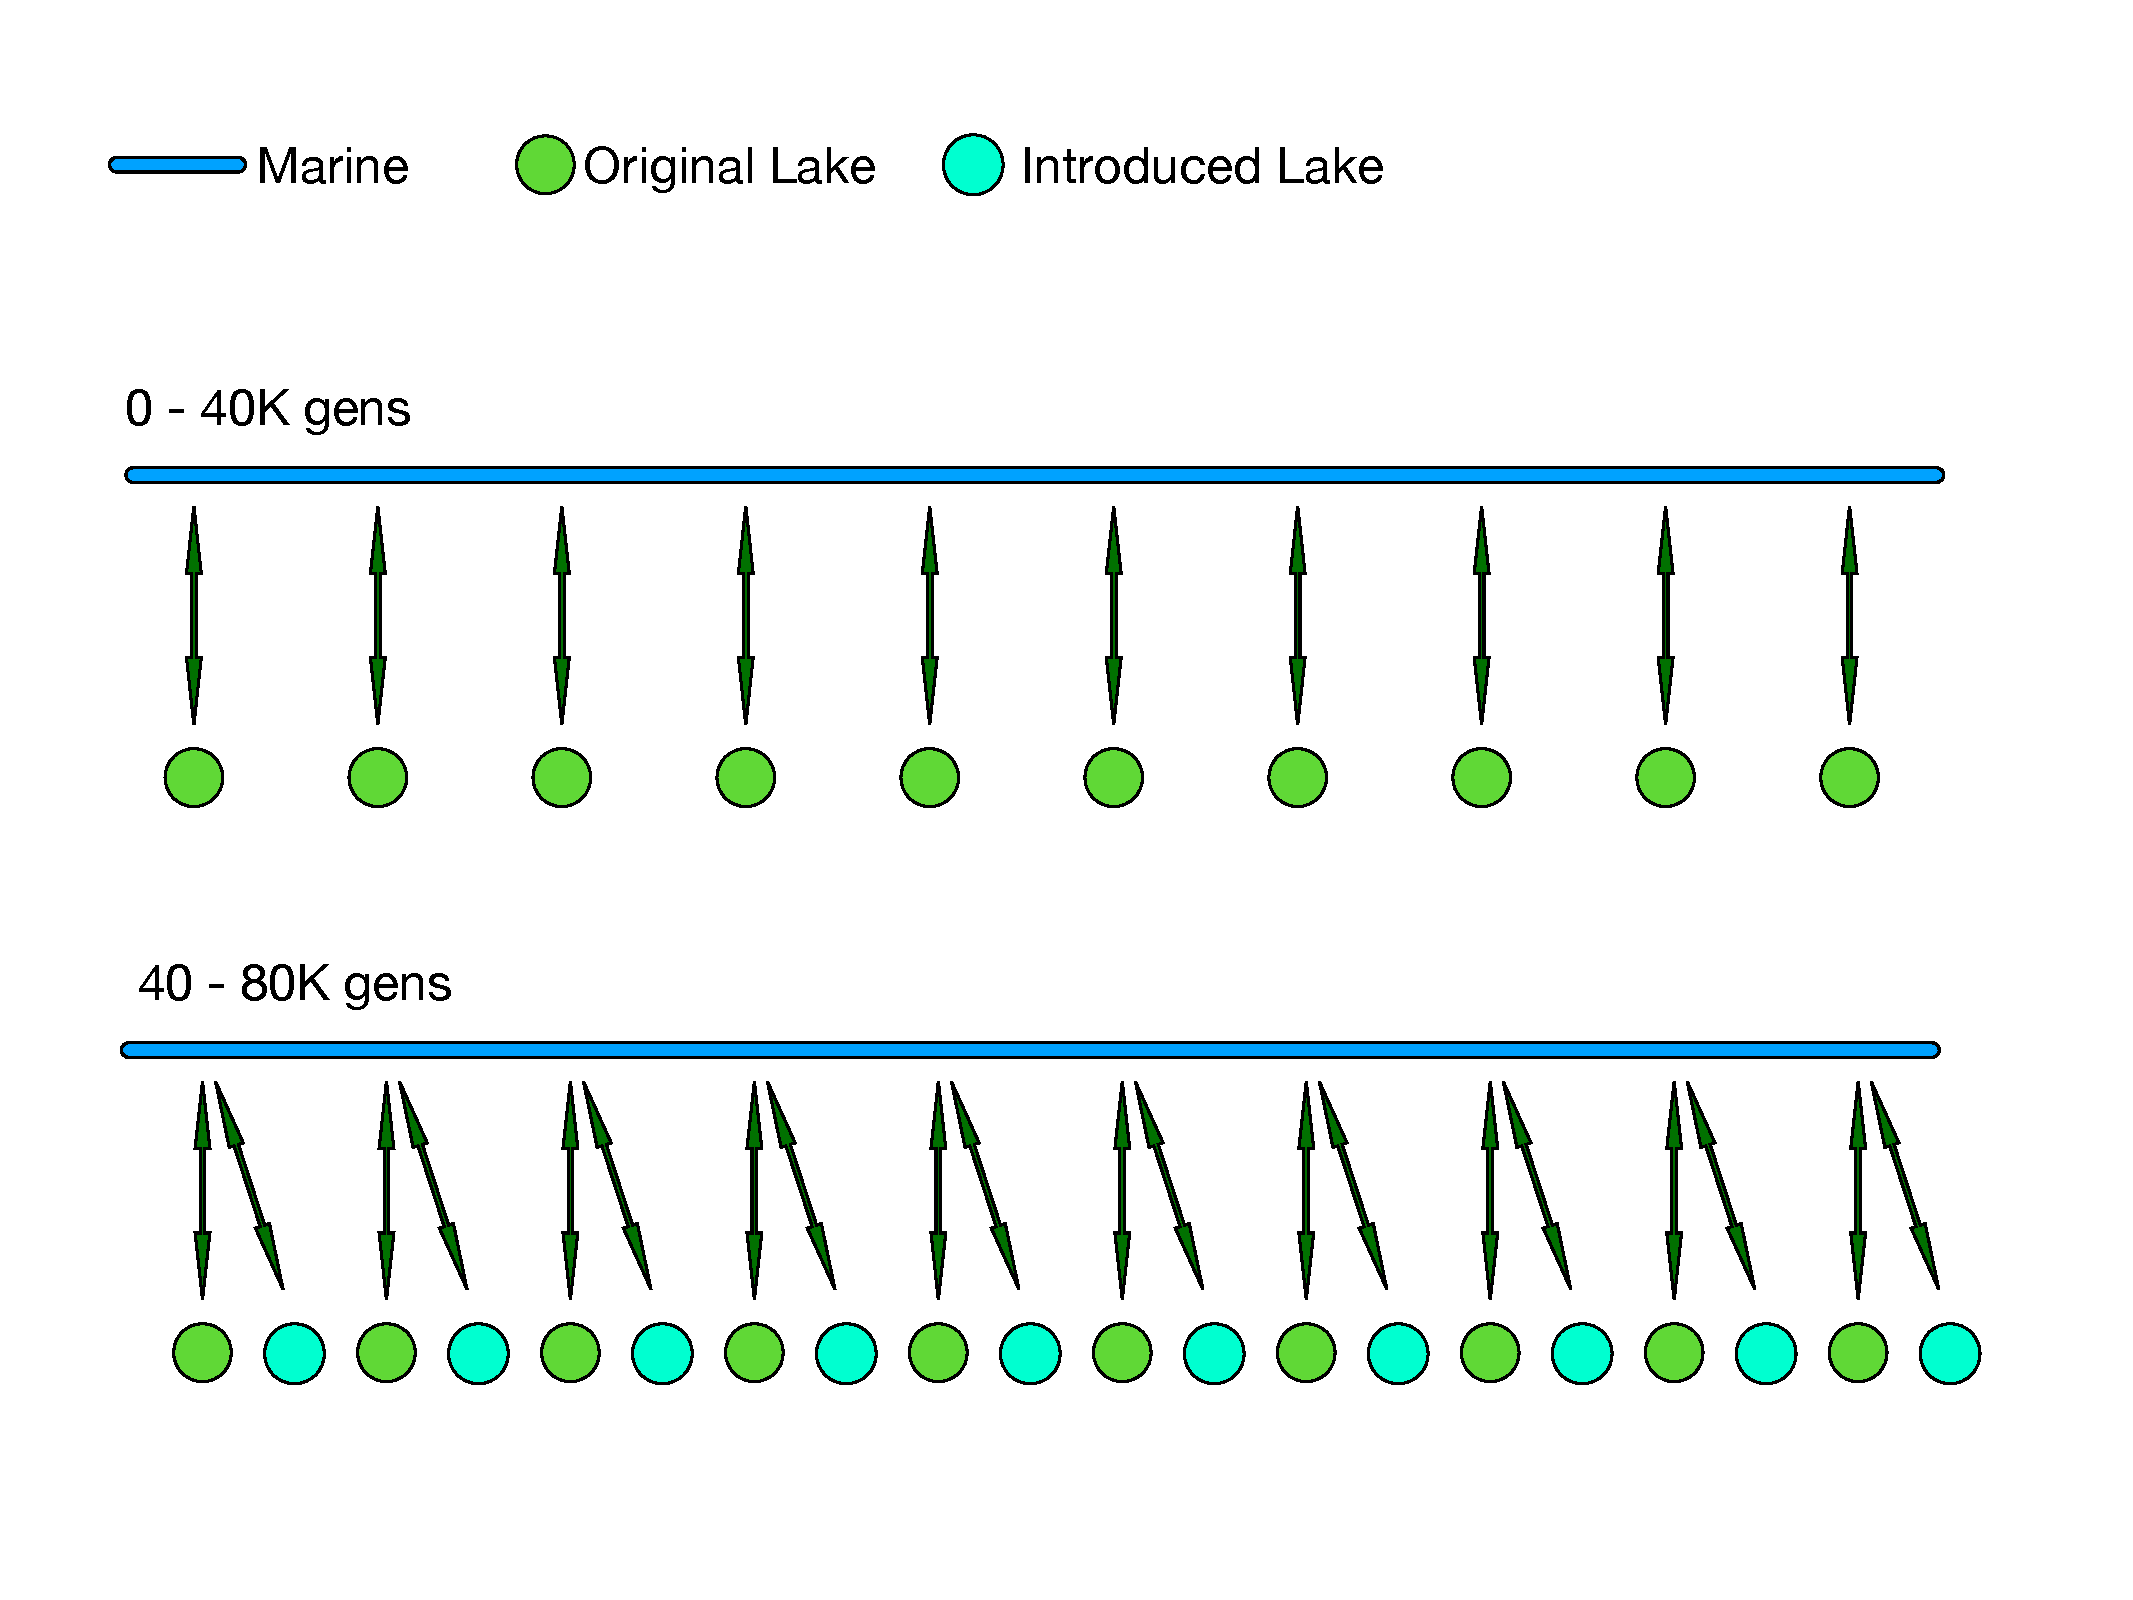
\includegraphics[width=0.6\linewidth]{GeographyDiagram}
  		\caption{A representation of the geographic and evolutionary history of all populations throughout the simulation. 
		The marine is a one-dimensional, continuous population with spatial positions ranging from [0.0 - 10.0]. 
		Each freshwater lake$_{i}$ for both the introduced and freshwater populations
		is a discrete population connected by migration only through the marine, at position $i - 0.5$. 
		The introduced lakes have the same spatial location (but separate?) and selective pressure as the original lakes, but arise at 40K generations.
		The marine has $2000$ diploid individuals while each of the lakes fluctuate around $200$. 
		the introduced population is initialized as a copy of all marine individuals to model marine 
		individuals inhabiting a newly created freshwater environment such as the ponds around Middleton Island.
		We then observe the selection process of marine individuals and following generations 
		with the new selective pressure across a range of parameter values. 
		%Migration between the marine and original lakes is 
		%set to $0$ the generation before introduction to avoid direct migrants from original $->$ introduced lakes.
		}
  		\label{fig:Geo}
	\end{center}
\end{figure}

\subsection*{Potential Genomic Architecture}

In SLiM, the genome is conceptually a linear array of loci defining locations for 
mutations that arise and breakpoints for recombination. 
Genomic elements define a range depicting the types of mutations that can arise, and the ratio at which different mutation types can arise. 
Although still uncertain about how much of the genome is directly associated with the distinguished phenotypes, 
GWAS has indicated clusters of loci (linkage groups? Operon?) along the genome to be causative. 
To mimic this and compare dynamics of neutral vs. effect under selection, 
we create regions of effect. (???)
In these genomic elements of effect, we uniformly allow additive, recessive, and dominant, mutation that can push phenotype in either the positive or negative direction to arise. 
Every genomic position outside of these effect regions only allows for selectively neutral mutations to arise.

In our simulations, there are 10 effect regions of size 100 loci, uniformly placed between buffer regions of size 4950 loci. 
This means the effect regions make up exactly $1\%$ of the entire genome for every individual throughout the simulation. 
The entire genome has a mutation rate of $10^{-7}$ meaning approximately 1 in every 100 individuals, per generation, is subject to a new mutation. 
The genome has a recombination rate of $10^{-5}$, which is approximately 1 breakpoint event, per individual, per generation. 

\subsection*{Selective Pressure}

%(TALK ABOUT ADAPTEDNESS and TRADE-OFF), 
% abstracting real fish phenotype with `` trait value "

%Trait value is equal to the sum of the contribution of the effect loci and the loci may be 
%add, dom, recc. Uniformly chosen 

To emulate the freshwater and marine selective pressure, 
we set up a quantitative genetics model in which fitness is phenotypically based. 
phenotype for an individual that is heterozygous at locus $H$
and homozygous derived at loci $D$ is $x = \sum_{\ell \in H} h_\ell s_\ell + \sum_{\ell \in D} s_\ell$,
where $h_\ell$ is the dominance coefficient for locus $\ell$ (0 for recessive, 1 for dominant, 0.5 for additive),
and $s_\ell$ is the effect of the derived mutation on the phenotype

Freshwater and Marine environments are distinguished by a single numeric value. 
This number is the optimum trait value for each environment
and acts as a representation of lateral plate number and opercle shape in the stickleback populations.
%The fitness of an individual is then determined by a probability density for a normal distribution 
%at the quantile (?) of the difference between the optimum and the individual's phenotype
We use a Gaussian fitness function, 
where the fitness of an individual with trait $x$ in a population with optimal trait value $x_0$ is:
\begin{align}
    f(x; x_0) &= \exp\left(\frac{(x - x_0)^2 }{ 2 \sigma^2}\right),
\end{align}
with $\sigma = 15$.


\subsection*{Descriptive statistics}

Here, we're interested in observing how different parameter values
(mainly migrations rates and recombination rates)
impact the sharing of alleles between populations. 
We define pre-existing freshwater adapted alleles at time $t$,
to be a mutations with a frequency higher than $0.5$ in \textit{any} of the original lakes, 
while remaining lower than $0.5$ in the marine. 
They are defined this way because the transportation hypothesis does not specify where or when an advantageous mutation arises,
but simply suggests that when a freshwater adapted alleles comes to high enough frequency, it too, could participate in the transportation process \citep{schluter2009genetics}.
To observe transportation of freshwater alleles in our simulations, we use a variety of metrics when sampling.
let $P_{1}$ and $P_{2}$ be the vector of mutation frequencies in the first and second populations, respectively.
with $\hat{P} = (P_{1} + P_{2}) / 2$ and
$PQ = (P_{1} \times (1 - P_{1}) + P_{2} \times (1 - P_{2})) / 2$,
we compute $F_{ST} = 1 - (PQ / (\hat{P} \times (1 - \hat{P})))$.
%mean number of original lakes each FAA appears in,
%and total number of unique FAA. 
Time to adaptation ($T_{adapt}$) of the introduced population is the generation at which
the difference between the average phenotype of the original and the introduced freshwater populations is less than 0.5. 
To understand where, as well as how much, of these pre-existing freshwater adapted alleles are being transported,
we track the the average percentage of freshwater adapted alleles at time $t$ across all populations throughout the simulation.


\section{Results}

Across a range of historical introgression from $\approx 0.01 - 100.0$ migrants per generation in populations of 
size 2000 diploid individuals, we encountered large influence on 
time to adaptation,
sharing of pre-existing freshwater adapted alleles,
and population genetic signals left behind in the simulated populations.
More gene flow is experienced with greater historical introgression between the two selective pressures.
Interestingly, the ability for separate populations to locally adapt to their own selective pressure was relatively unaffected 
until the highest rate of migration between the marine and freshwater environments.
All rates of historical introgression aside from the lowest, helped both the initial and introduced freshwater populations 
share pre-existing freshwater adapted alleles.
The sharing of alleles resulted in rapid adaptation ($\approx 100$ generations) of the introduced population (split from the marine population) to adapt to the freshwater environment.
We also found that larger amounts of migration allow for more statistical power and less false positives in the resulting population genetics data ($F_{st}$ per SNP across the genome).

\begin{figure}
	\begin{center}
  		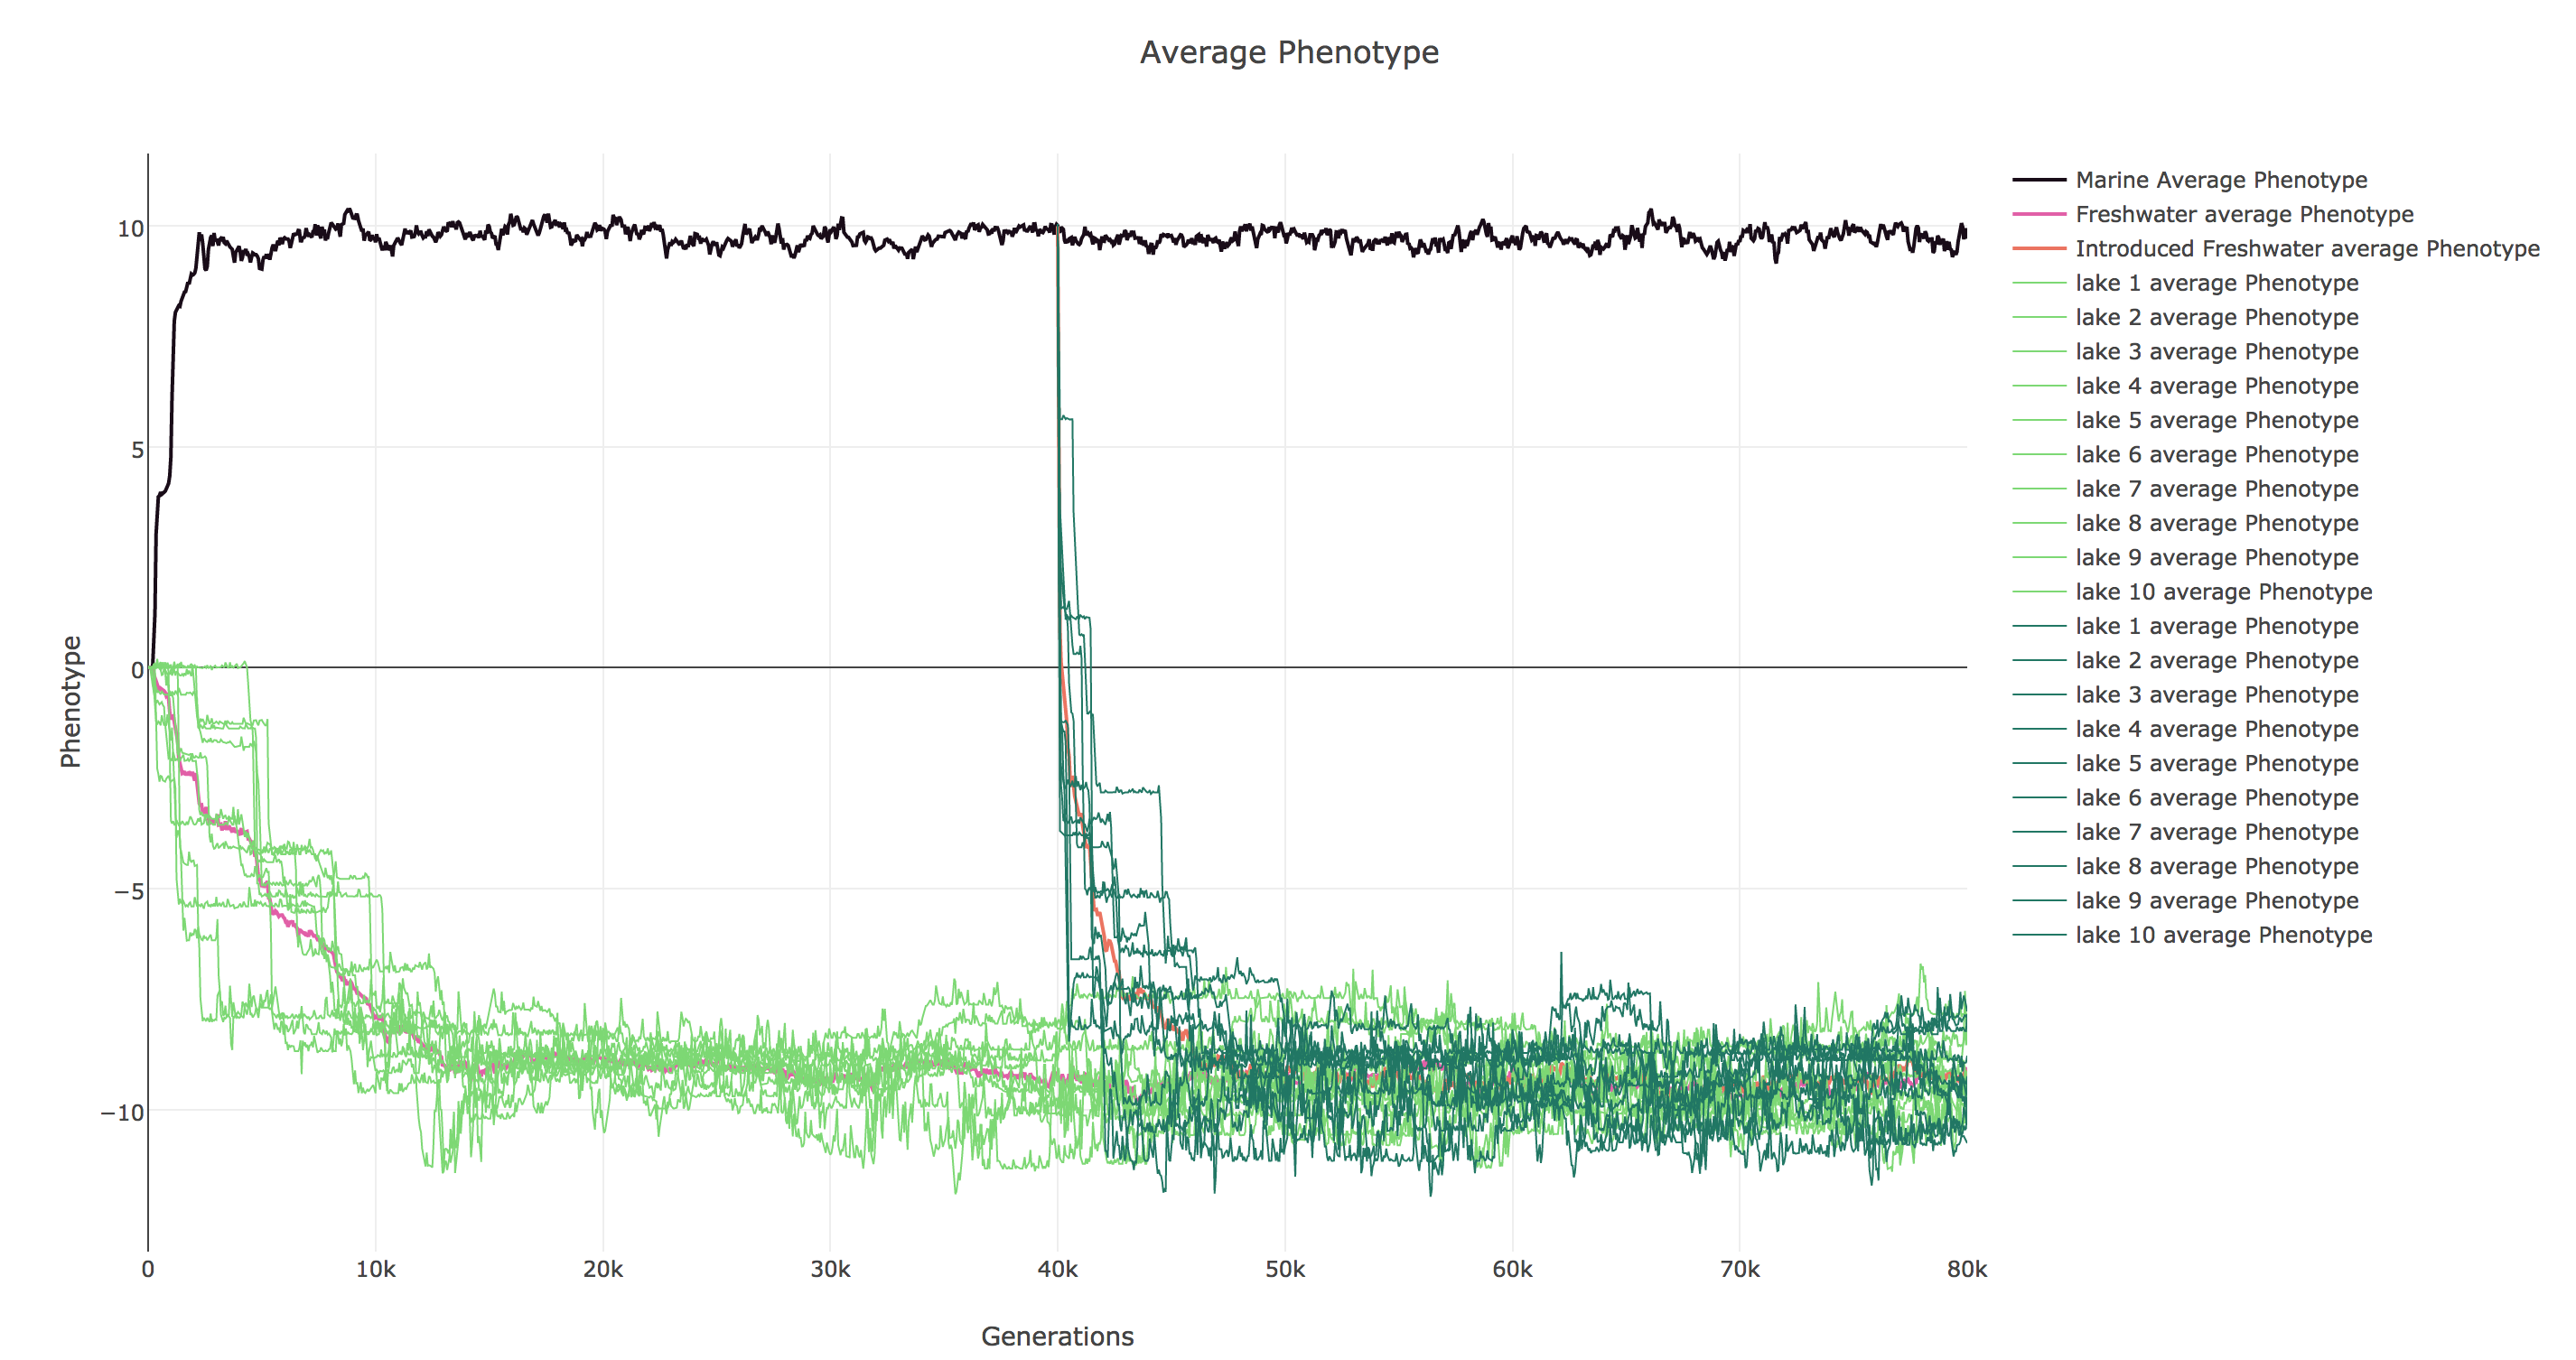
\includegraphics[width=0.7\linewidth]{plotlyPlots/PhenotypeThroughout5e-4.png}
  		\caption{ Mean individual trait value in each population as a function of time $t$, in generations. 
		This is a single simulation run at a migration rate of $5 \times 10^{-4} \approx 1$ mig/gen in both 
		directions for every freshwater population to the single marine population. 
		The dark black line represents the mean phenotype of the single marine population with an optimum trait value of + 10. 
		The pink represents the entire initial freshwater population mean
		of all the lakes (light green) with and optimum trait value of -10.
		The orange represents the entire introduced freshwater population mean
		of all the lakes (dark green) with an optimum trait value of -10 as well.
		}
  		\label{fig:phenotype_ts2}
	\end{center}
\end{figure}

\begin{figure}
	\begin{center}
  		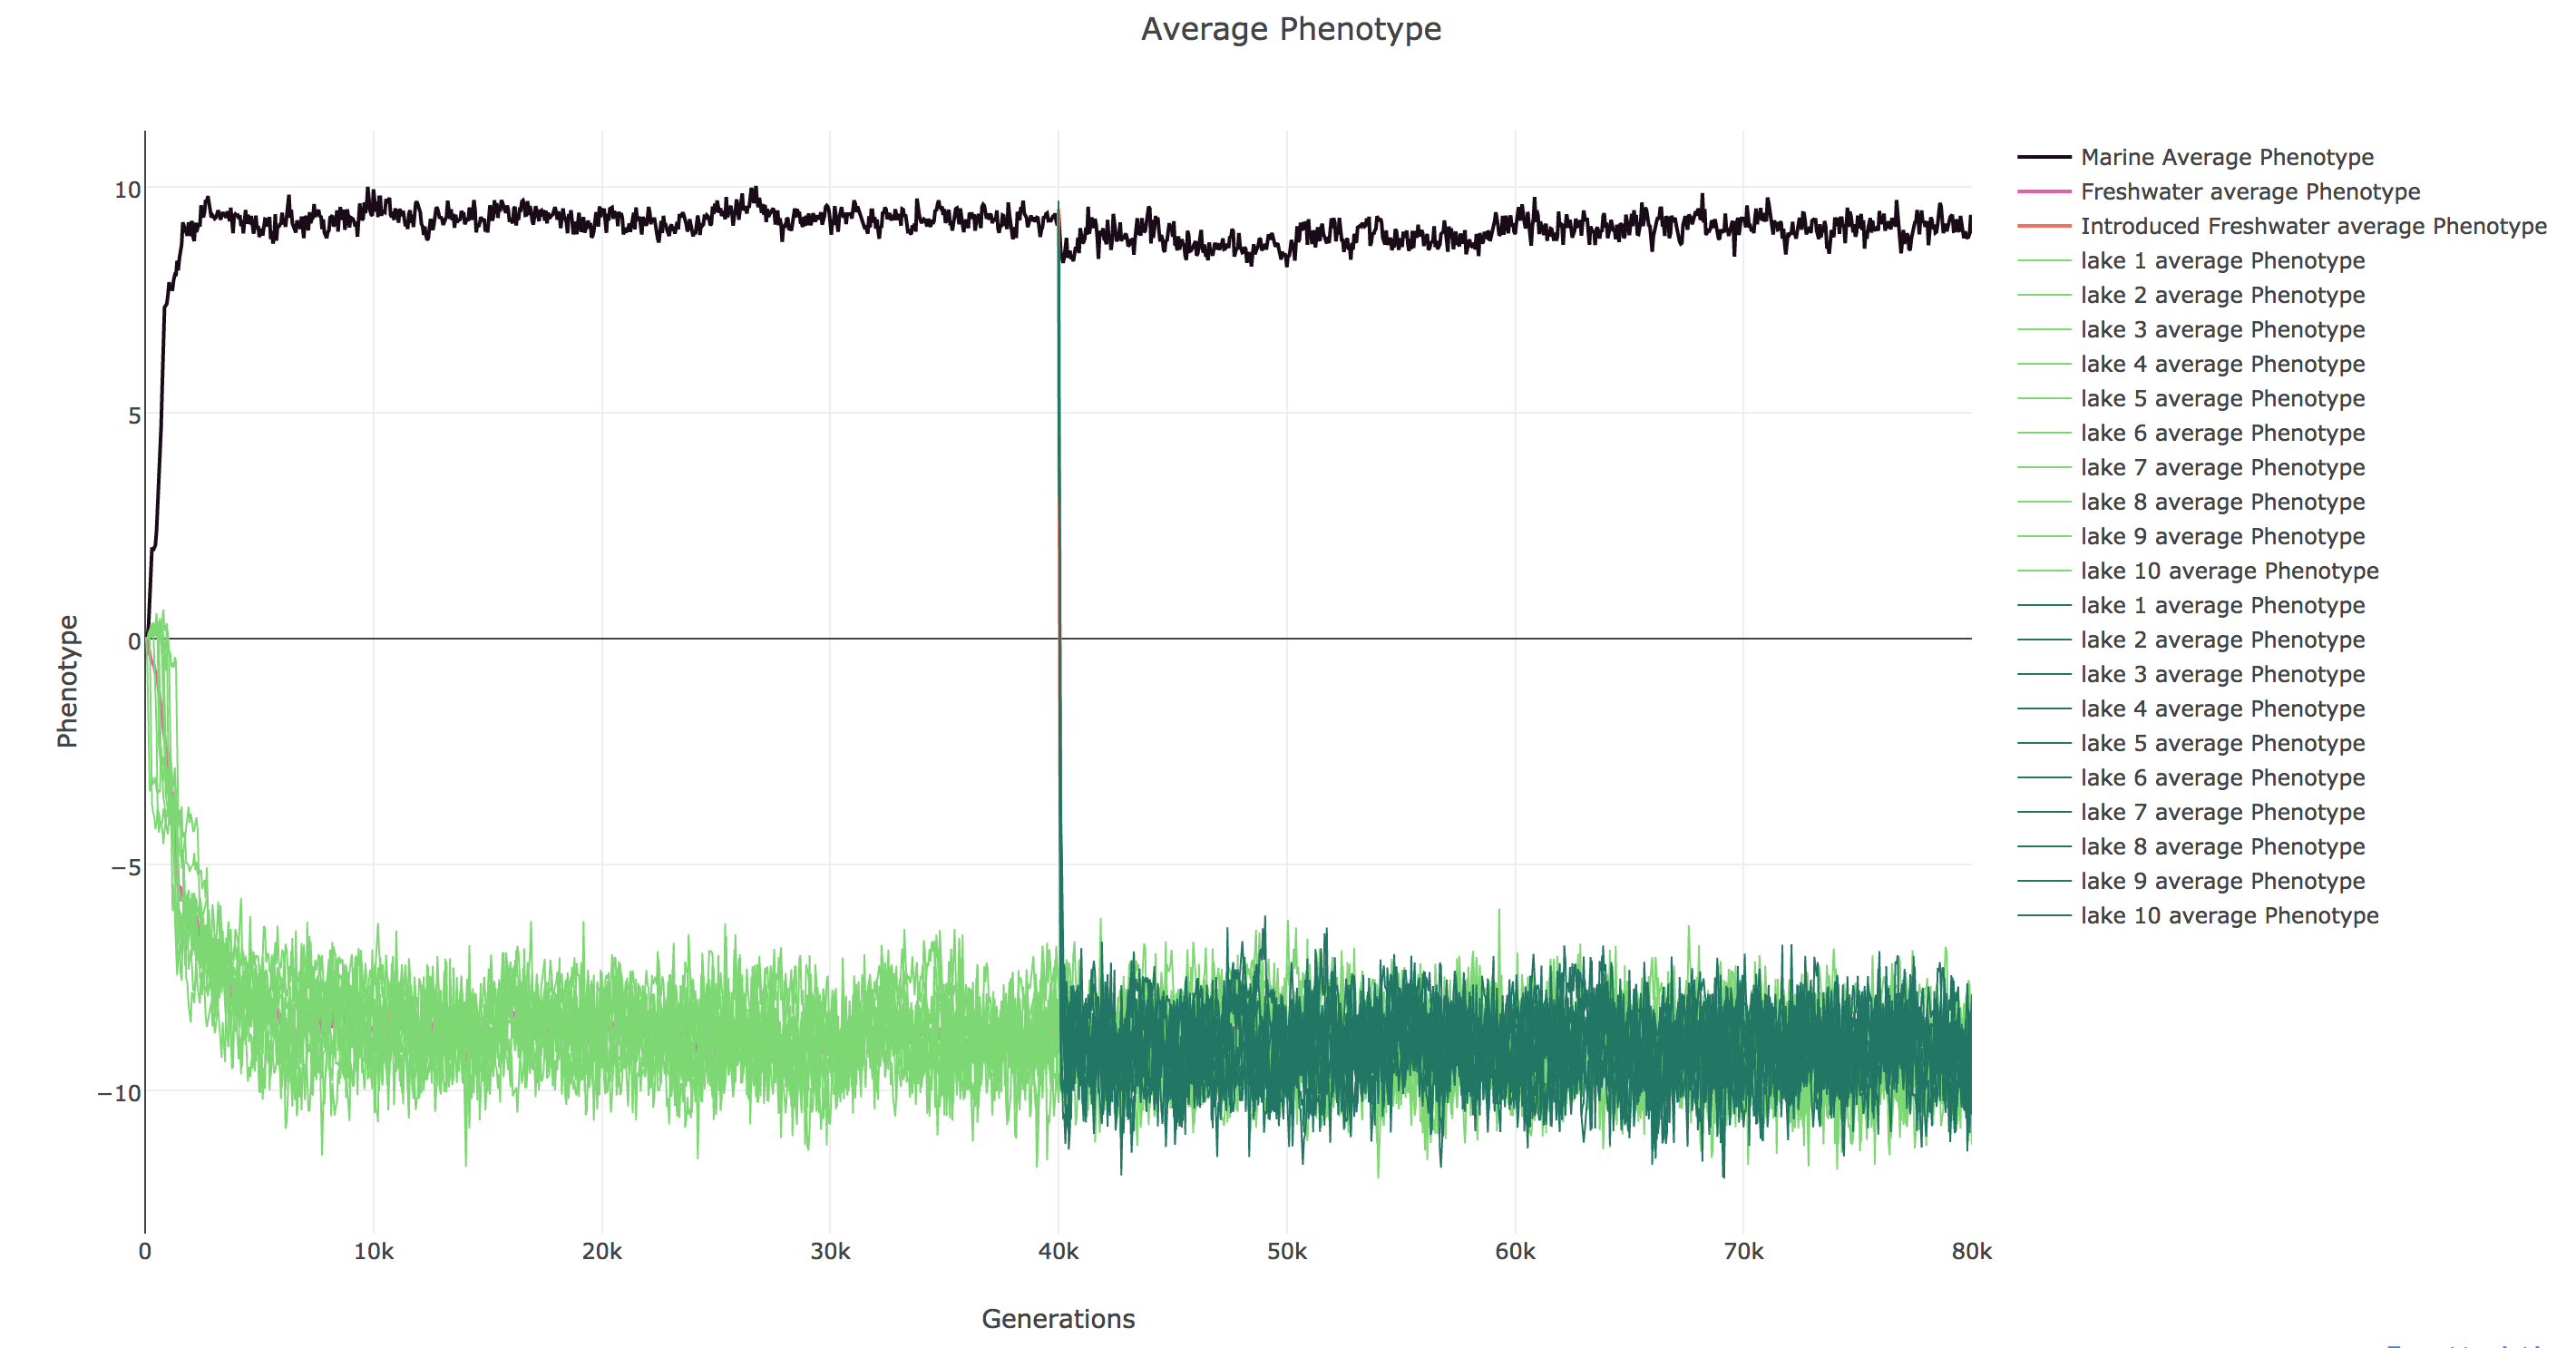
\includegraphics[width=0.7\linewidth]{plotlyPlots/PhenotypeThroughout5e-3.png}
  		\caption{Mean individual trait value in each population as a function of time $t$, in generations. 
		This is a single simulation run at a migration rate of $5 \times 10^{-3} \approx 1$ mig/gen in both 
		directions for every freshwater population to the single marine population. 
		The dark black line represents the mean phenotype of the single marine population with an optimum trait value of + 10. 
		The pink represents the entire initial freshwater population mean
		of all the lakes (light green) with and optimum trait value of -10.
		The orange represents the entire introduced freshwater population mean
		of all the lakes (dark green) with an optimum trait value of -10 as well.
		}
  		\label{fig:phenotype_ts3}
	\end{center}
\end{figure}

\jgg{we should make one caption and the two above should be top-bottom sub-figures}
\jgg{also, interesting point to make on second plot, you can see the initial lakes taking the same size step. sharing}
%I could zoom in on the relevent portions of the figure for this. (begging and introduction)
% a 2 by 2 with the important sections (0 - 20K) $ (40-50K) for both above figures. share axes
%\jgg{finished with most edits up to here}

\subsection*{Local Adaptation: differentiation with gene flow}

%Talk about the genetic basis of trait. 
%Talk about the progression of adaptation. How you can see introduction new alleles

Local adaptation occurred across all simulated parameter values.
Starting from the same baseline, freshwater and marine populations diverged phenotypically
until they reached an equilibrium
where the population means were close to or at the optimal phenotype. 
The distribution of mean number of freshwater adapted alleles suggested that there was 
$\approx 8$ SNPs underlying the freshwater phenotype. 
This was true for all rates of introgression except for the highest at $100$ mig/gen
where the mean trait value in the populations equilibrated well below the optimum.
We can see the introduction of new alleles in Figure \ref{fig:phenotype_ts2}. 
In generation (0 - 20K) The sweeps that cause jumps in the mean phenotype of the freshwater population 
have a relatively large effect size equal to or greater than $1$.
%In Figure \ref{fig:counts} we can see that the number of effect regions with zero 
%pre-existing freshwater adapted alleles increased with introgression while
%regions of effect containing more pre-existing freshwater adapted alleles increase.
Phenotypic variation within each population was small compared to the difference between populations.
Polymorphic loci that impact the individual trait value,
showed greater differentiation compared to neutral loci between marine and freshwater populations, 
with the exception of the lowest migration rate of 0.01 migrants per generation per lake. 

\todo{ add more general observations and caveats about not all parameter values. }
\plr{It would be nice to have a small table of parameter values,
    so that when someone wonders ``What was the population size again?'' they could easily find it.}
\jgg{Re: agreed}

\subsection*{Migration homogenizes genetic variation}

%FIGURES THAT SHOW THIS:
%- Fst Plots.
%- SGV Plots.
%- Haplotype plots

\begin{figure}
	\begin{center}
  		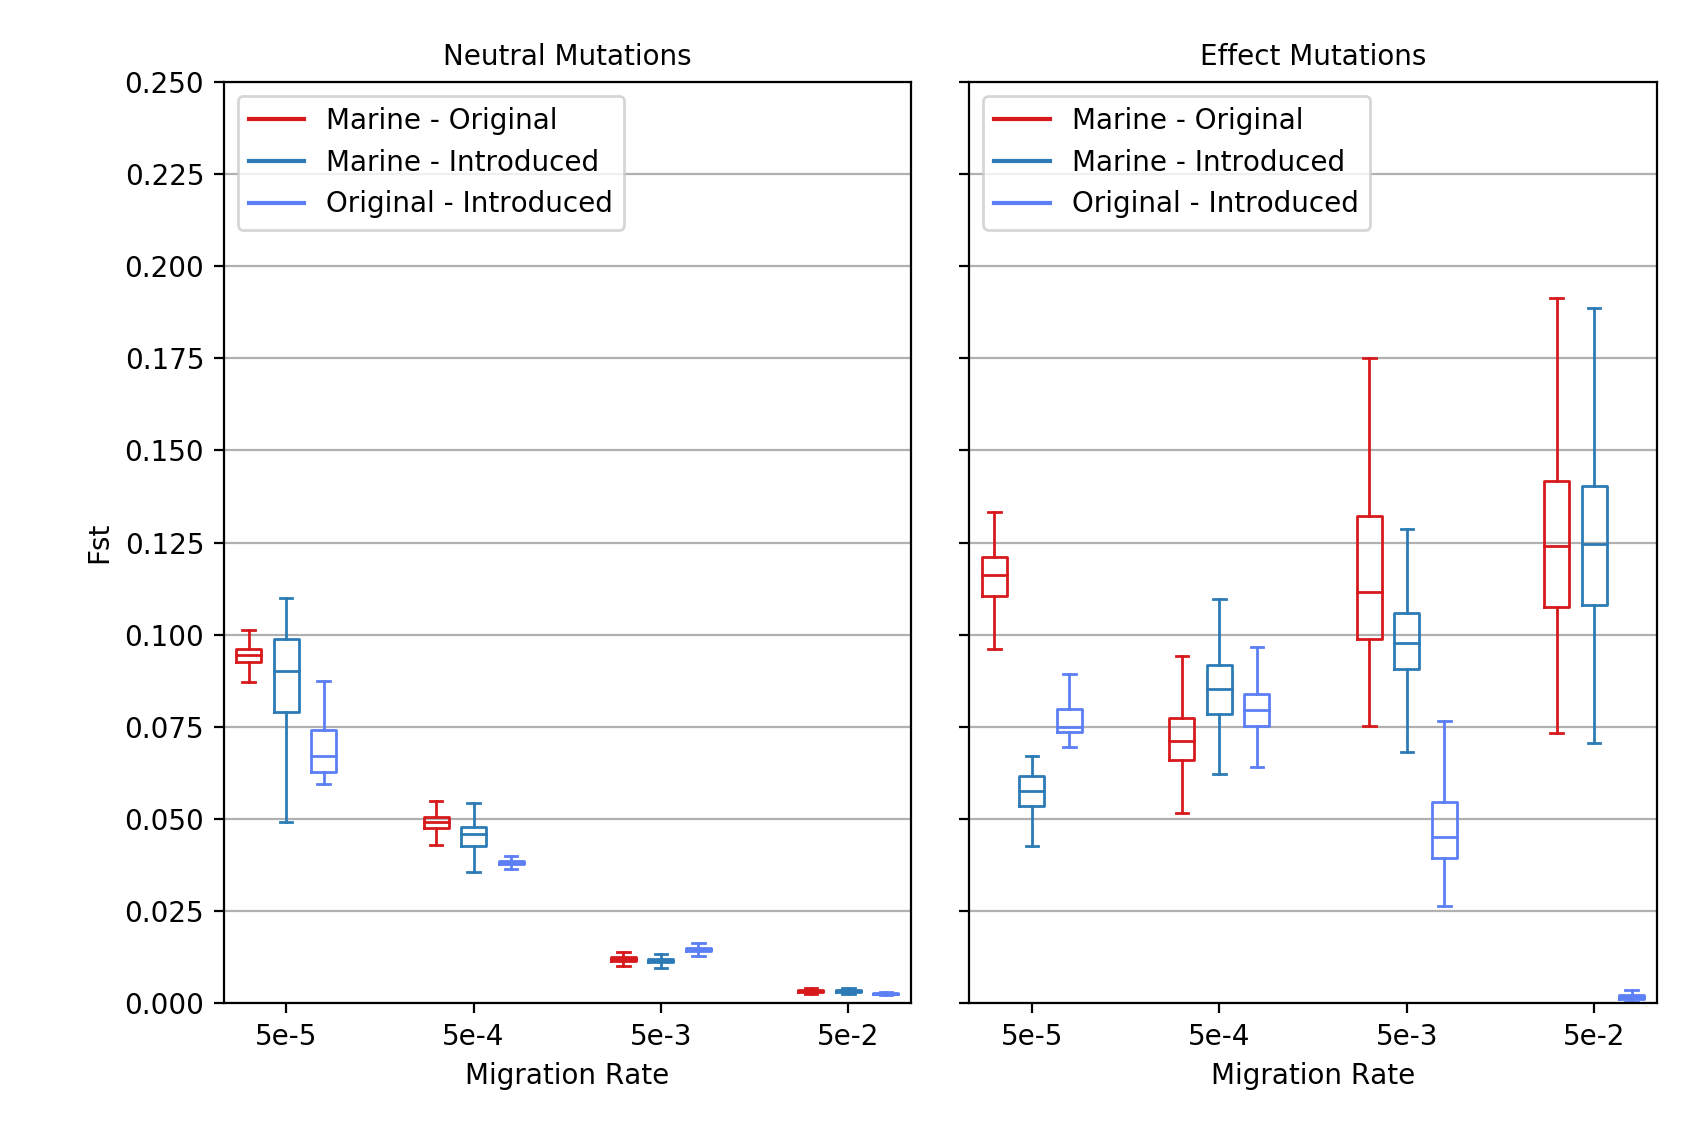
\includegraphics[width=0.8\linewidth]{matplotlibPlots/FST_HRR.png}
  		\caption{Distributions of $F_{st}$  values between the three subpopulations throughout the simulations.
		On the left, $F_{st}$ was calculated only on neutral mutation frequencies. On the right, $F_{st}$ was calculated
		only on effect (Impact on phenotype) mutation frequencies. 
		Effect mutations are acted upon by selection as they have an affect on fitness where neutral mutations  }
  		\label{fig:Fst}
	\end{center}
\end{figure}

Across increasing parameters of migration, we observed more gene flow across the populations. 
As can be seen in Figure \ref{fig:Fst},
$F_{st}$ values for neutral alleles steadily decline between all sets of populations as 
migration increases, this illustrates less difference between sections of the genome which are not acted
upon by selection, in all populations.
Additionally, standing genetic variance
(seen in Figure \ref{fig:SGV})
values in the marine population steady increased with migration which suggests that more alleles from the 
lakes surrounding were exporting alleles into the marine individual.

%TIES TO NATURE?
%SPECIFICALLY (interesting stuff)

\subsection*{migration affects the speed of adaptation}

%FIGURES THAT SHOW THIS:
%-Time to adaptation
\begin{figure}
	\begin{center}
  		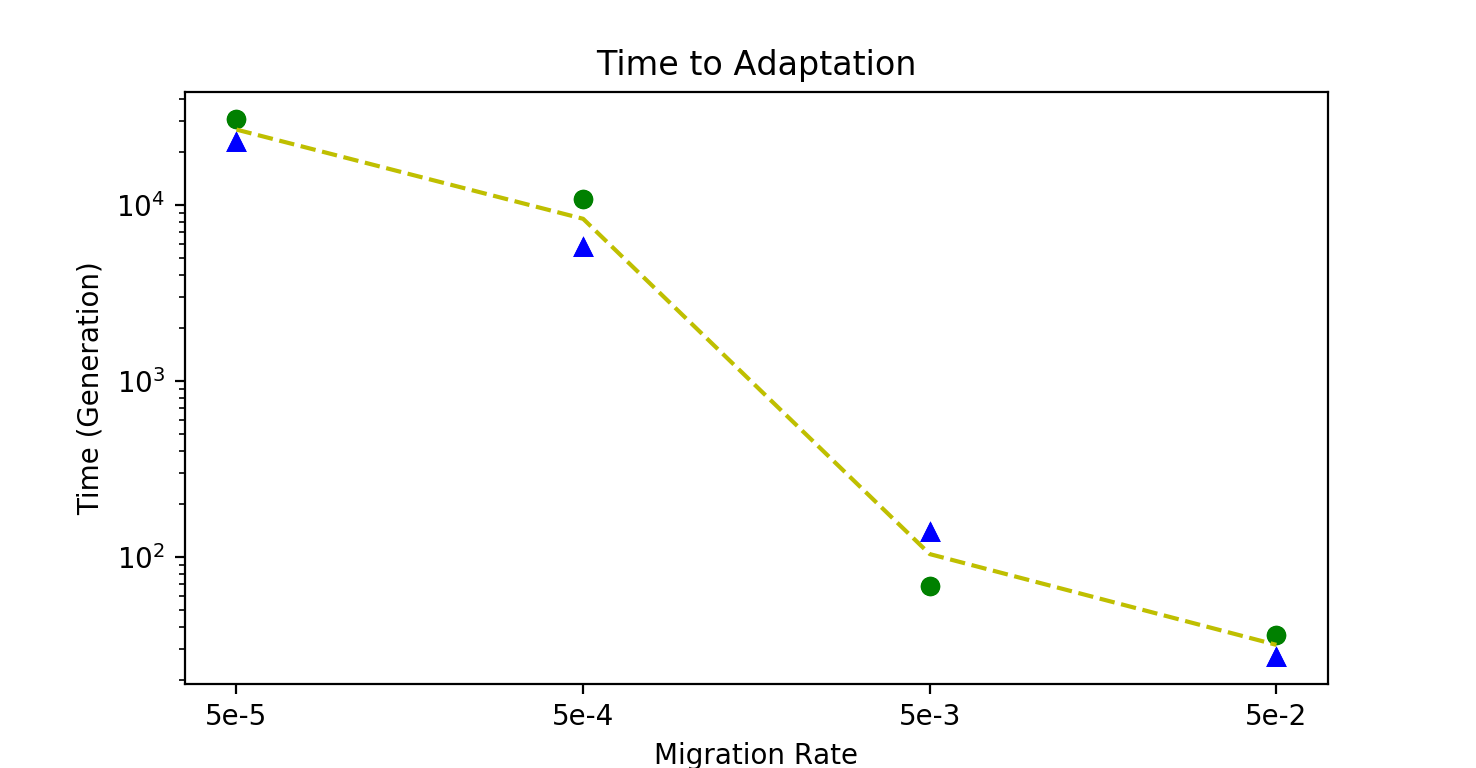
\includegraphics[width=0.8\linewidth]{matplotlibPlots/TimeToAdaptation.png}
  		\caption{Time to adaptation as a function of migration rate ($M$) parameter value. This is where we measure how many generation
		it takes for the introduced population's mean phenotype to come within 0.5 of the original lakes average phenotype. 
		Each point represents a simulation run at some value of $M$. 
		The yellow dashed line is the average of all points at each respective parameter value}
  		\label{fig:TimeToAdaptation}
	\end{center}
\end{figure}

We observed a dramatic shift in time until adaptation for the introduced populations
as migration rates increased. 
As can be seen in Figure \ref{fig:TimeToAdaptation} at the lowest migration rate of $5 \times 10^{-5}$,
It took the introduced population over 20 thousand generations for the mean trait value, $X_{I}$ of all the lakes to 
get to within 0.5 of the original lakes mean trait value, $X_{O}$
%\plr{From the plots it looks more like adaptation happens (at least in most lakes) by like 10K or 15K.}
This suggests that selection was acting primarily on new mutations, and that the 
introduced lakes needed to wait for a beneficial mutation to arise before 
it was selected upon. 
%\plr{We should do the calculation to see if this makes sense: 
%    there's one new effect mutation in the right direction every 100 generations in the lakes,
%    one of effect size $s$ has probability of about $s/2$ of not being lost to drift...}
In Figure \ref{fig:MPFAI} we can see there was a correlation between the amount of pre-existing freshwater adapted alleles in the 
marine and the rapid adaptation of the introduced populations. 
In the same figure we can see the distributions
for both the original and Introduced freshwater population become more balanced (similar?) as introgression increases.
This is further evidence that the introduced population is taking advantage of the alleles from the initial freshwater populations



%(2) Do the math, discuss number ( and possibly type ) of mutations underlying the trait value.

%TIES TO NATURE?
 
\subsection*{sharing of freshwater adapted alleles}

%FIGURES THAT SHOW THIS:
%-MPAA / IND
%-Total/Avg shared
\begin{figure}
	\begin{center}
  		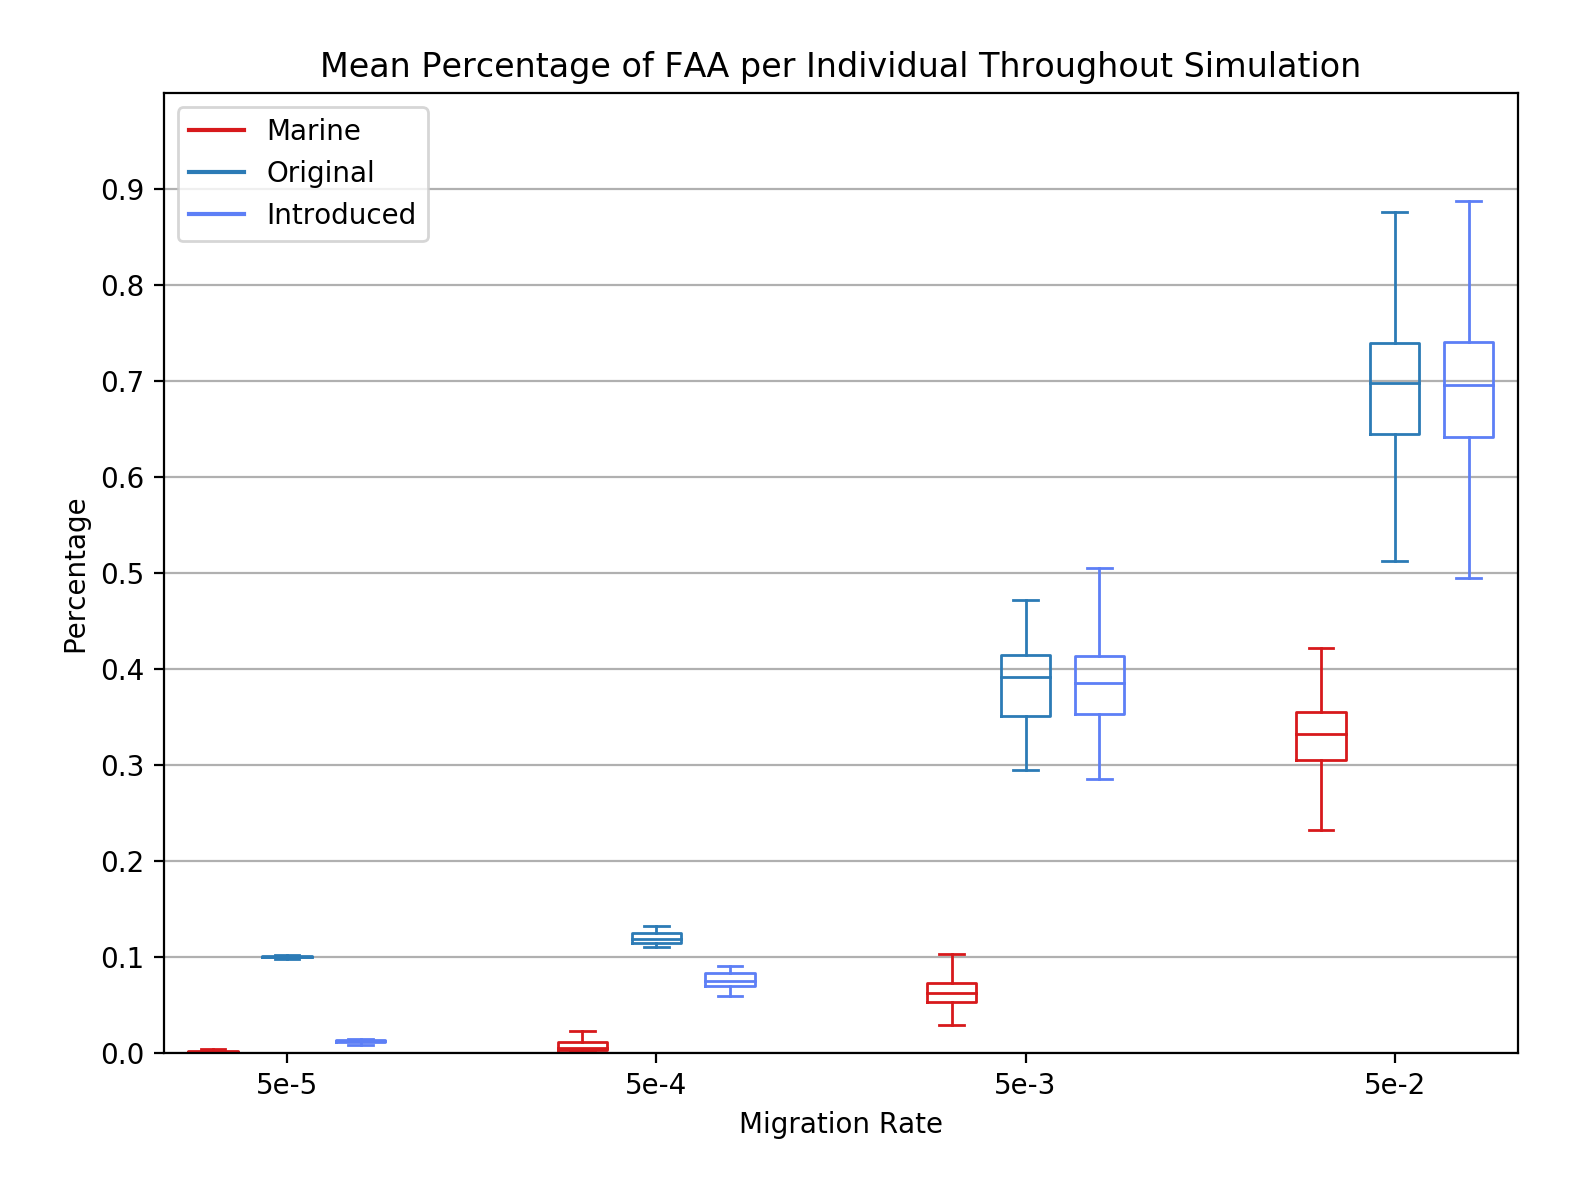
\includegraphics[width=\linewidth]{matplotlibPlots/MPFAI.png}
  		\caption{Distributions of mean percentage of freshwater adapted alleles (FAA) per individual throughout the simulation run, for each subpopulation.
		We count the total number of freshwater alleles for each individual before averaging them in each population and dividing by the total number of defined
		freshwater adapted alleles.
		Looking at total number of FAA per individual gives us an idea behind how many alleles underly a freshwater haplotype, 
		while the percentage tells us the variance of the haplotype}
		\label{fig:MPFAI}
	\end{center}
\end{figure}

To further investigate this correlation, we take a look at the freshwater adapted alleles driving 
local adaptation of the introduced population. 
One common metric we investigate is the percentage of freshwater adapted alleles per individual in each of the populations, at any time $t$. 
This gives us a idea of where the where these alleles are being distributed throughout the simulation run. 
Looking at the lowest migration rate for the original lakes population In Figure \ref{fig:MPFAI}
We see that the average individual has almost exactly $1/10^{th}$ of the total defined freshwater adapted alleles throughout the simulation. 
Because FAA are defined among \textit{any} population, this suggests that each one of the $10$ 
lakes has created their own solution to adaptation of the the freshwater selective pressure. 

As we can see in Figure \ref{fig:NumFAA}
as historical introgression increases for the simulations, 
we see the distribution of the total number of freshwater adapted alleles decrease, and 
the average number of lakes each allele appears in at high frequency ($p > 0.5$), increase.
With the distribution of effect size remaining the same across all simulations, 
these are both suggestive of the original lakes sharing solutions to the same selective pressure.

%TIES TO NATURE?

%SPECIFICALLY (interesting stuff)

\subsection*{do the math}
\jgg{peter? :)}

(1) - What is the mean fitness of a population 

(2) - assuming everybody is at the mean fitness, what is the expected num of offspring after t gens in marine

(3) - expected num of establishing alleles in new lake. = (num outmigrants) $\times$ (num per outmigrant) $\times$ (prob migrant) $\times$ $2\hat{x}s $ mean fit in new lake

\subsection*{We see Migration Load after a certain threshold of migration}

%FIGURES THAT SHOW THIS:
%- Phenotype Distribution
\begin{figure}[h!tb]
	\begin{center}
  		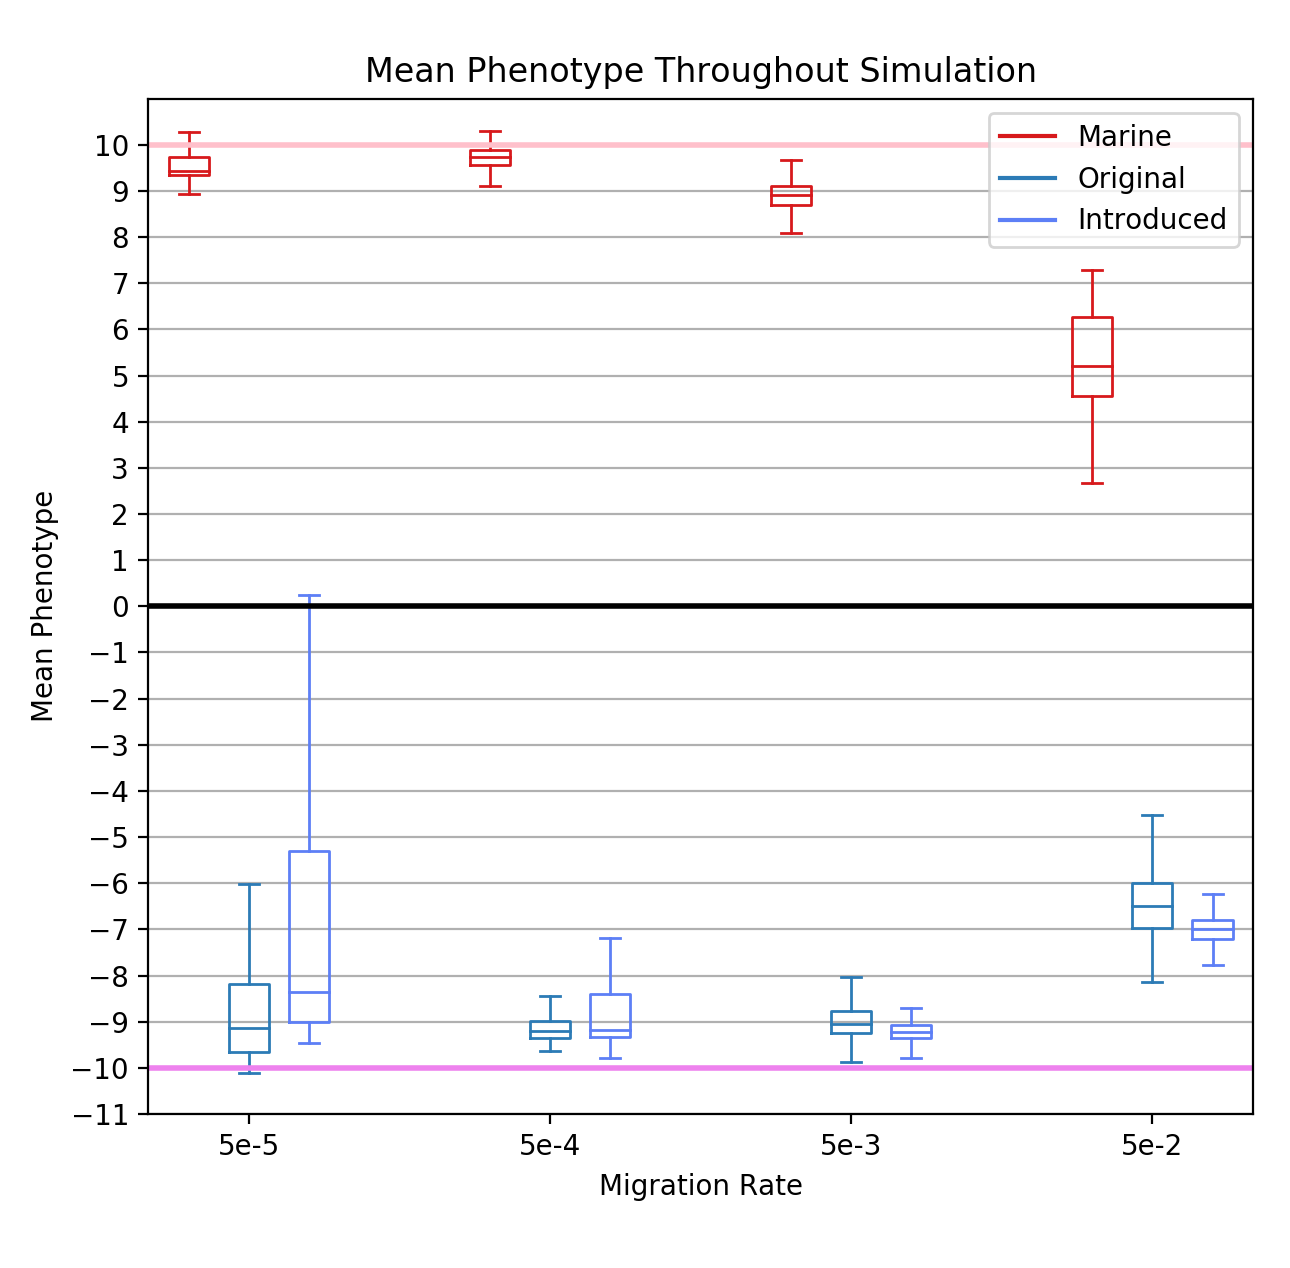
\includegraphics[width=0.6\linewidth]{matplotlibPlots/MeanPhenotype1.png}
  		\caption{Distribution of mean phenotype throughout simulation runs at separate migration rate ($M$) parameter values, for each population.
		The dashed pink line (Pheno = +10) is the optimum phenotype any individual in the marine environment.
		In contrast the purple line at (Pheno = -10) represents the optimum for any individual in the freshwater environment. 
		All individuals at generation 0 (beginning of the simulation) 
		}
  		\label{fig:MeanPhenotype}
	\end{center}
\end{figure}

%GENERAL

In the distributions we have shown across migration rate parameter values, 
We have experienced the most dramatic shifts of the population dynamics at $M = 5x10^{-3}$.
After a threshold between this and $M = 5x10^{-2}$, all populations begin to experience migration load. 
Significant gene flow constricts local adaptation
as a consequence of a large number of offspring through hybridization events between subpopulations.
In Figure \ref{fig:MeanPhenotype} at $M = 5x10^{-2}$, we can see the distribution of average phenotype throughout the simulation
pull towards the opposing selective pressure value and away from the local optimum trait value in all populations.

%TIES TO NATURE?

%SPECIFICALLY (interesting stuff)

\subsection*{Realized genomic architecture and signals}


\begin{figure}
	\begin{center}
  		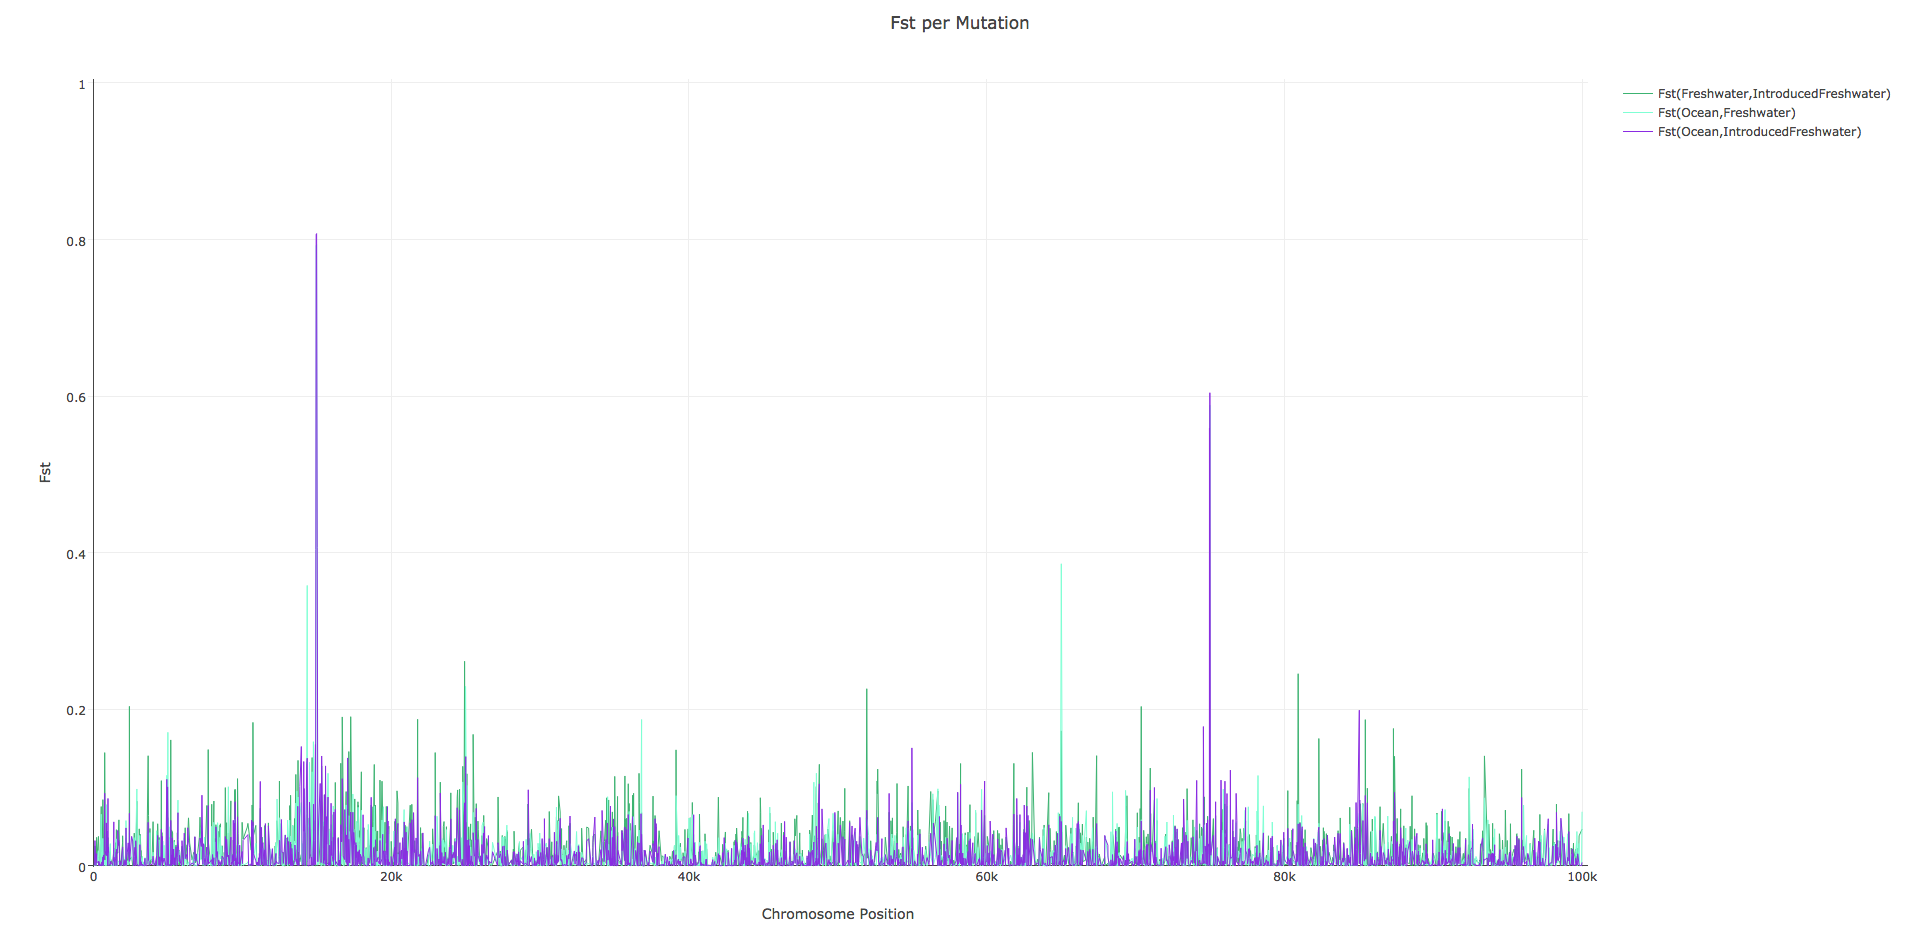
\includegraphics[width=0.7\linewidth]{plotlyPlots/FstAcross5e-3.png}
  		\caption{(Description and cleaning needed)
		}
  		\label{fig:Fst3}
	\end{center}
\end{figure}

\begin{figure}
	\begin{center}
  		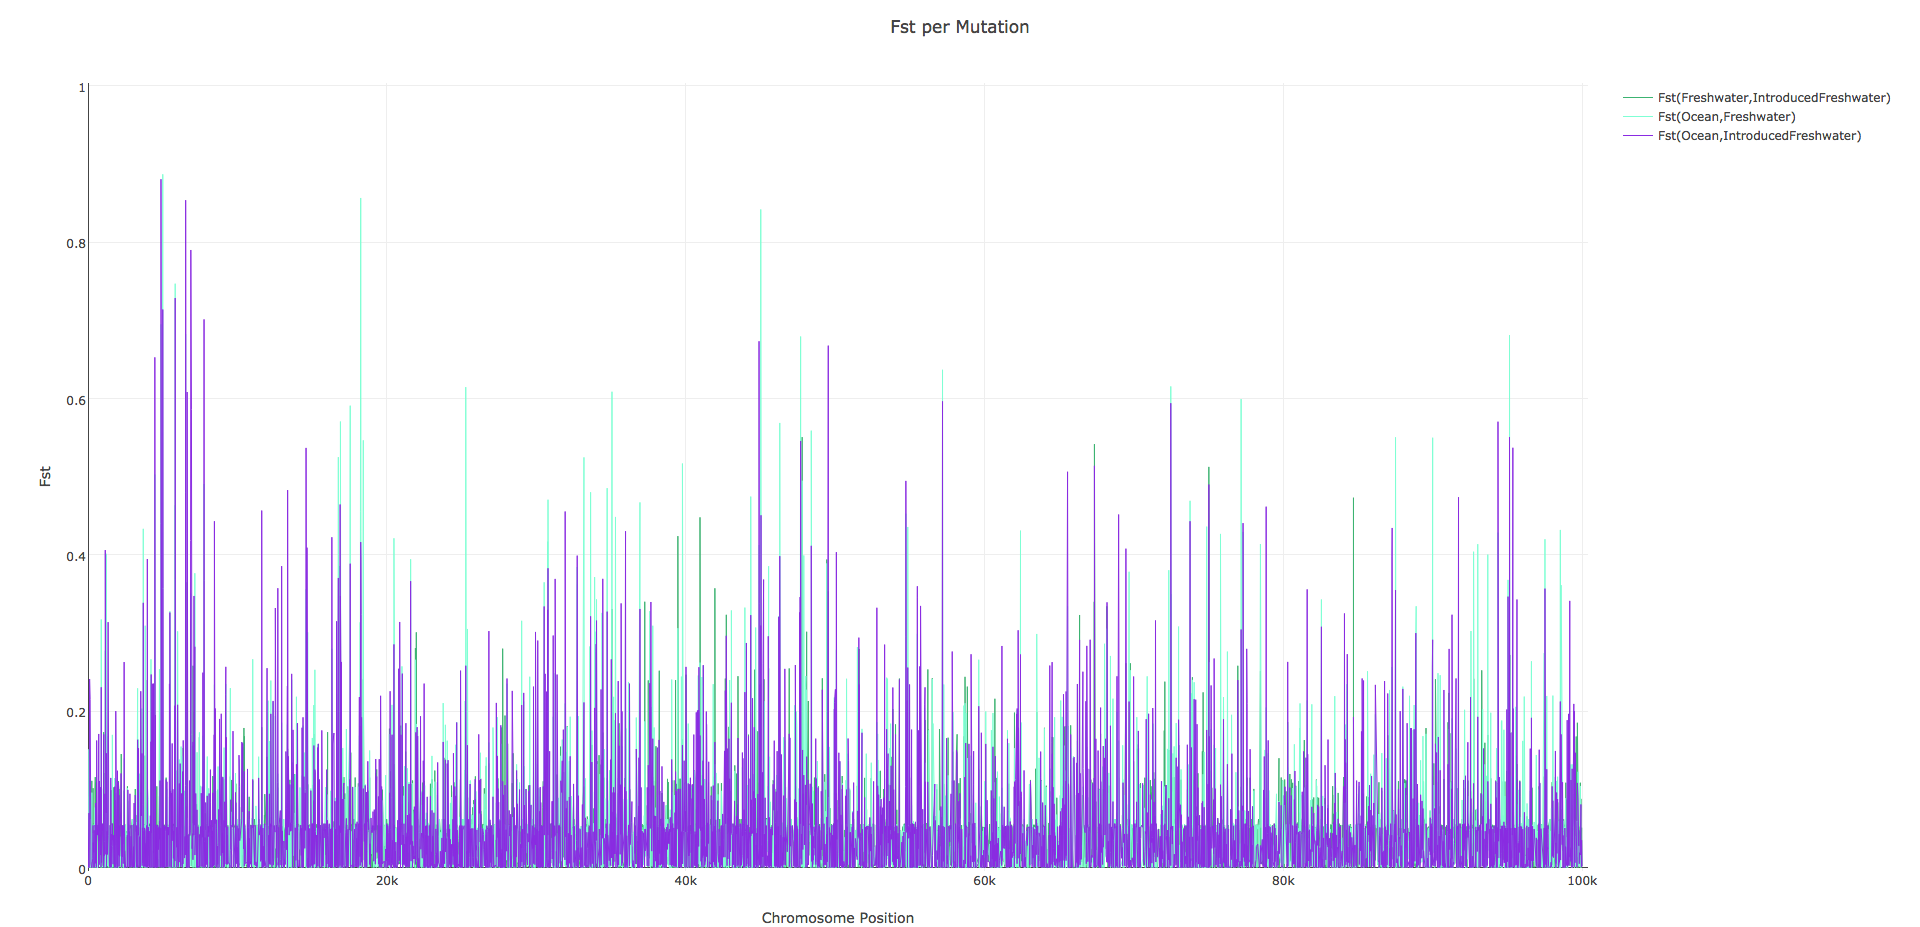
\includegraphics[width=0.7\linewidth]{plotlyPlots/FstAcross5e-4.png}
  		\caption{(Description and cleaning needed)
		}
  		\label{fig:Fst2}
	\end{center}
\end{figure}

Now we take a closer look at the genomic architecture of local adaptation between freshwater and marine individuals. 
Often when looking at real datas, biologists observe patterns of $F_{st}$ and clustering of alleles that suggest causative loci for certain traits.
However, researchers would like to know how parameters such as migration and recombination impact the results from natural populations.
To give an idea about the impact of these parameters in our model, we examine the distribution, location, and false positive rate on predicting effect loci
given the $F_{st}$ per SNP across the genome. 


\begin{figure}
	\begin{center}
  		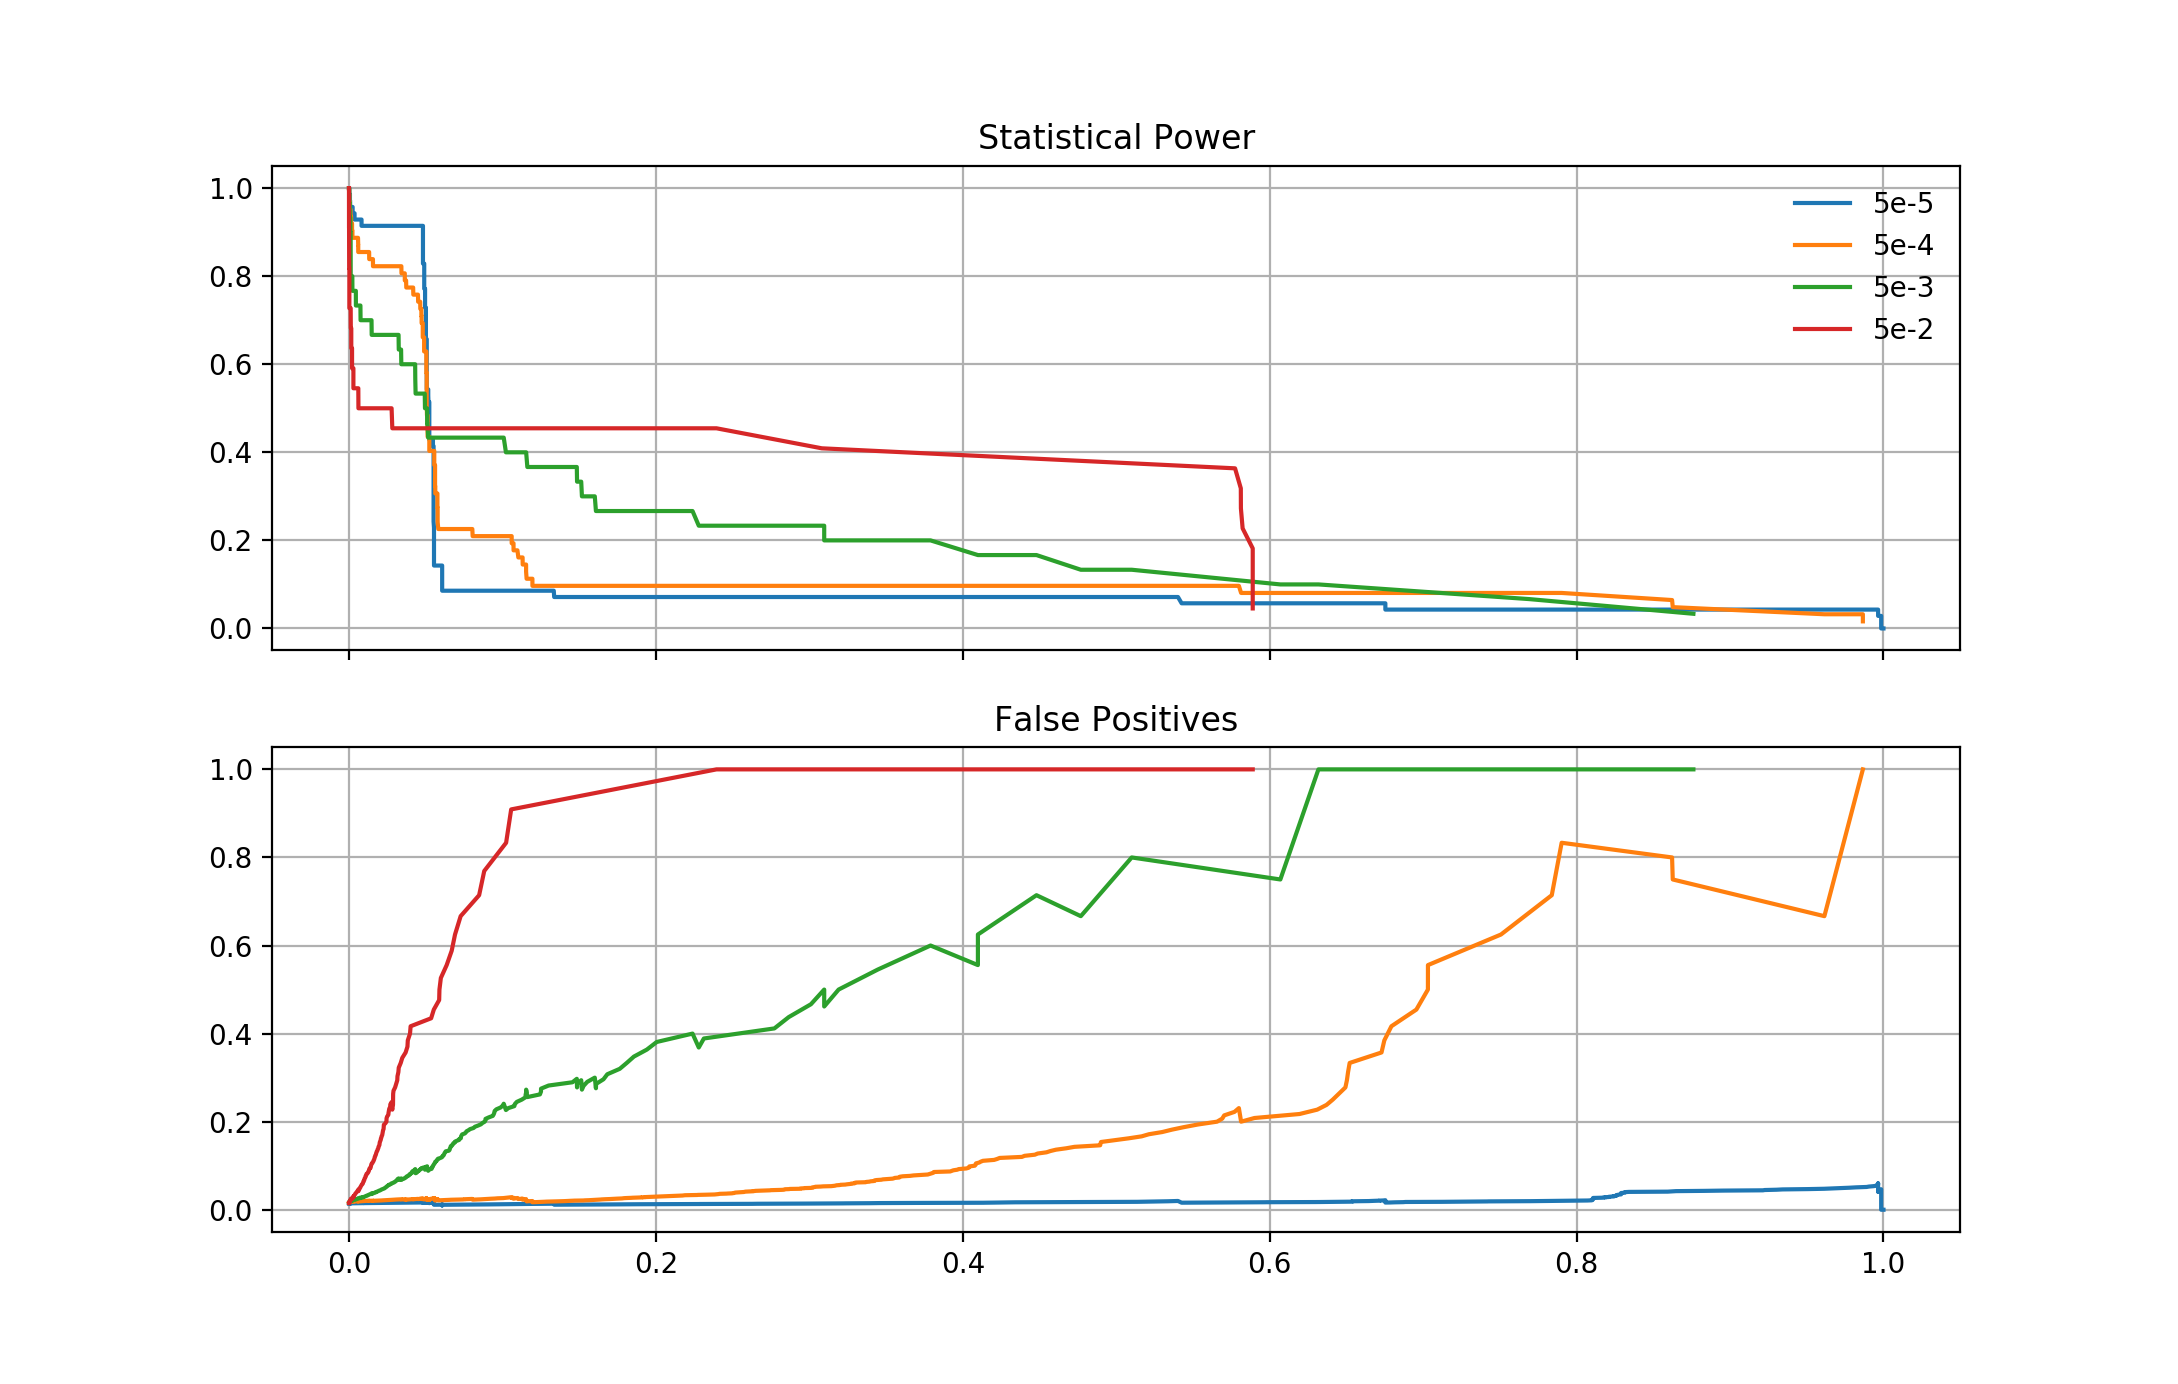
\includegraphics[width=0.7\linewidth]{matplotlibPlots/Power_FP.png}
  		\caption{ 
		%SP - suppose you have an Fst Peak, how likely is it that that region is causal. 
		Statistical Power and False Positives as a function of $F_{st}$ threshold. 
		Statistical Power is the likelihood that a SNP will be predicted to have an effect on phenotype when there is an effect to be detected (?).
		False Positives give us the ratio of SNPs that effect phenotype to total SNPs greater than the $F_{st}$ threshold.
		}
  		\label{fig:Power_FP}
	\end{center}
\end{figure}

%Suppose you have a Fst Peak, ___ how likely is it that that region is causal. and conversely, what proportion of 
%the causal loci are under Fst Peaks.

\subsection*{False-Positives \& Statistical Power}

%\plr{Start off by talking about Fst along the genome, then say ``if we identify QTL as the outliers, then...''}
%\plr{I vote for combining and including figures \ref{fig:Fst2} and \ref{fig:Fst3}.}

At higher rates of introgression in our simulations, we saw $F_{st}$ peaks at regions of the genome underlying individual trait value (phenotype). 
In contrast, the lower rates of introgression showed higher $F_{st}$ across the entire genome such that the regions under selection were indistinguishable. 
For every $F_{st}$ peak, we saw the same regions of the genome express high $F_{st}$ when comparing either the initial \textit{or} introduced freshwater populations to the marine population.
If we identify quantitative trait loci as the outliers, then this is again suggestive of both freshwater populations sharing regions of divergence from the marine population.

With 10 effect regions across the genome, we can see in \ref{fig:Fst3} that only about 1 or 2 of the region contain peaks. 
%SOFT STATEMENT - MORE (Peak) EVALUATION?
When looking closely at the peaks we see that each is usually a composition of 7-8 SNPs close in proximity.
%SOFT STATEMENT -
Because some of those mutations are selectively neutral (we can see this because the counts of FAA are not as high as the number in the clusters),
this is suggestive of hitchhiking alleles along with the SNPs being brought to high frequency by a selective sweeps.


In regions of the genome underlying individual trait value, we observed 
Given that migration increases the gene flow between subpopulations, how valid are $F_{st}$ peaks at different $M$. 
Knowing exactly which mutations effect phenotype in our simulations, 
we can look at the statistical power and false positives given $F_{st}$ per SNP across the genome. 
In Figure \ref{fig:Power_FP} , looking at an $F_{st}$ threshold greater than 1, we see the two lowest migration rates $10^{-5}$ and $10^{-4}$ having very little statical power. 
This along with low false positive rate across all $F_{st}$ threshold values is fairly predictable when you consider the high $F_{st}$ values across the genome. 

%The lowest migration rate of $10^{-5}$ also has a very low false positive rate across all $F_{st}$ threshold values.
%\subsubsection*{Low Recombination Causes Clustering}

\section{Conclusion \& Discussion}

We have shown that historical introgression, at our given parameter sets,
is able to reproduce rapid and parallel adaptation similar to what we've seen in real populations such as Middleton island.
Selection is able to rebuild the freshwater haplotype from marine populations as a medium between all freshwater populations.
Almost all rates of migration were helpful in the efficiency of the population to locally adapt except for the highest at which migration load 
limited the ability of the populations to reach the local optimum. 

We also have also explored the genomic architecture as a consequence of the nature of selection in our scenario. 
The alleles underlying individual trait value were of large effect and a low number. 
With a total of $10^{5}$ loci, to be realistic, each loci should represent 1000 $Kb$ in real data.
\jgg{This should be expanded upon, not sure what this means in terms of the genomic architecture}

We have also shown introgression is beneficial for inferring causative loci from divergence ($F_{st}$) along the genome. 
This is generally because noise of selectively neutral alleles divergence can appear causative when genetic drift causes more 
differences between populations that have little gene flow between them.
It's important to know that in all scenarios, hitchhiking of selectively neutral alleles could also be 
mistaken for being causative as they often display the same amount of divergence.
%wouldn't it be cool if we could use this fact and simulate introgression, starting with real data that is noisy to extrapolate the areas we care about?
%this could be nonsense 

% at low M we should be able to predict something ---
% at high M we should be able to predict something ----

%Here, we suggest a range of migration rate (introgression) parameter values which would allow for the rapid (and in turn, parallel) adaptation 
%of marine stickleback introduced intro a freshwater environment.
%While this range is heavily effected by all other selections of parameter values. 

%(1) There's a threshold of introgression for both rapid adaptation and migration load. 
%(1.5) Maybe refer to the literature for migration load.  
\subsection*{thresholds}

We have found that too little migration leads to selection upon new mutations in all subpopulations and lakes alike. 
In contrast, at high migration rates we have seen that migration load limits 
the ability for species to locally adapt to the selective pressure of their environment.
This leads us to consider a window of introgression which allows for the transportation
of FAA's without migration load. 


\subsection*{connect results back to real data?}

%In a species that commonly is subjected to two general types of selective pressure 
%such as marine and freshwater stickleback this is suggestive of the benefit of hybridization in all subpopulations before
%reaching a point of pre or post zygotic 

%(3) discuss what signals researchers could possibly look out for or connect to real data


\clearpage
%\plr{some problems because you had bibliographystyle before bibliography}
\bibliographystyle{plainnat}
\bibliography{Citations}{}

\section{Supp.}

\begin{figure}
	\begin{center}
  		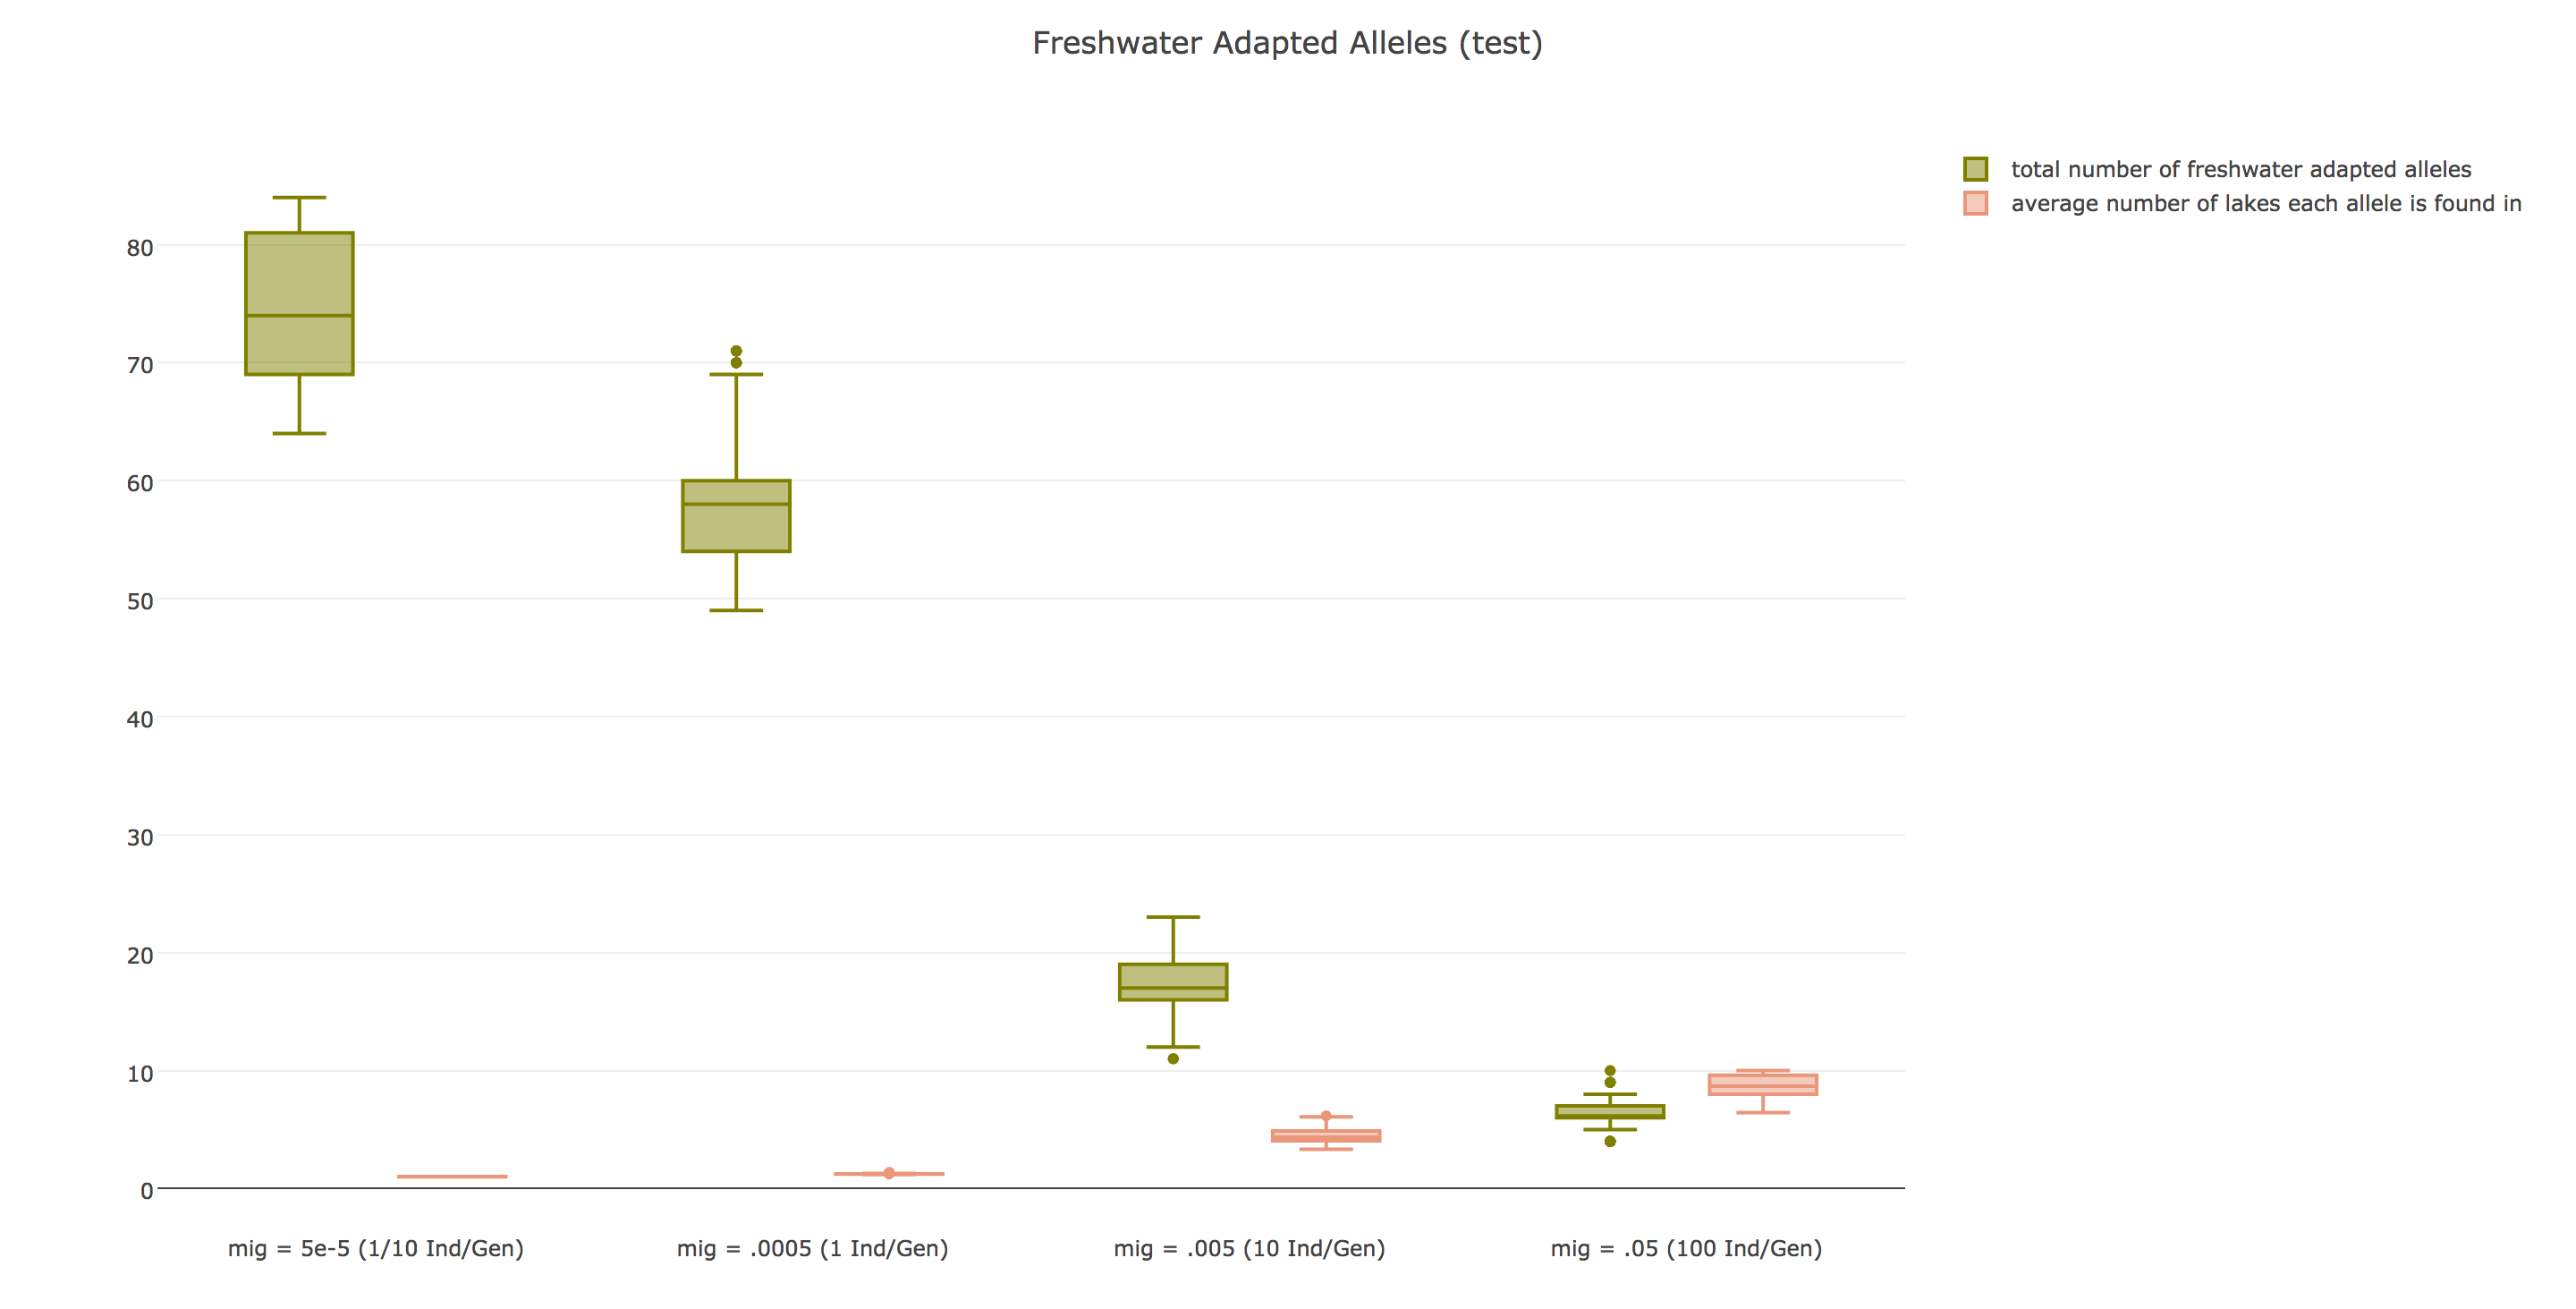
\includegraphics[width=\linewidth]{plotlyPlots/NumFAA.png}
  		\caption{(PLACEHOLDER)}
		\label{fig:NumFAA}
	\end{center}
\end{figure}

\begin{figure}
	\begin{center}
  		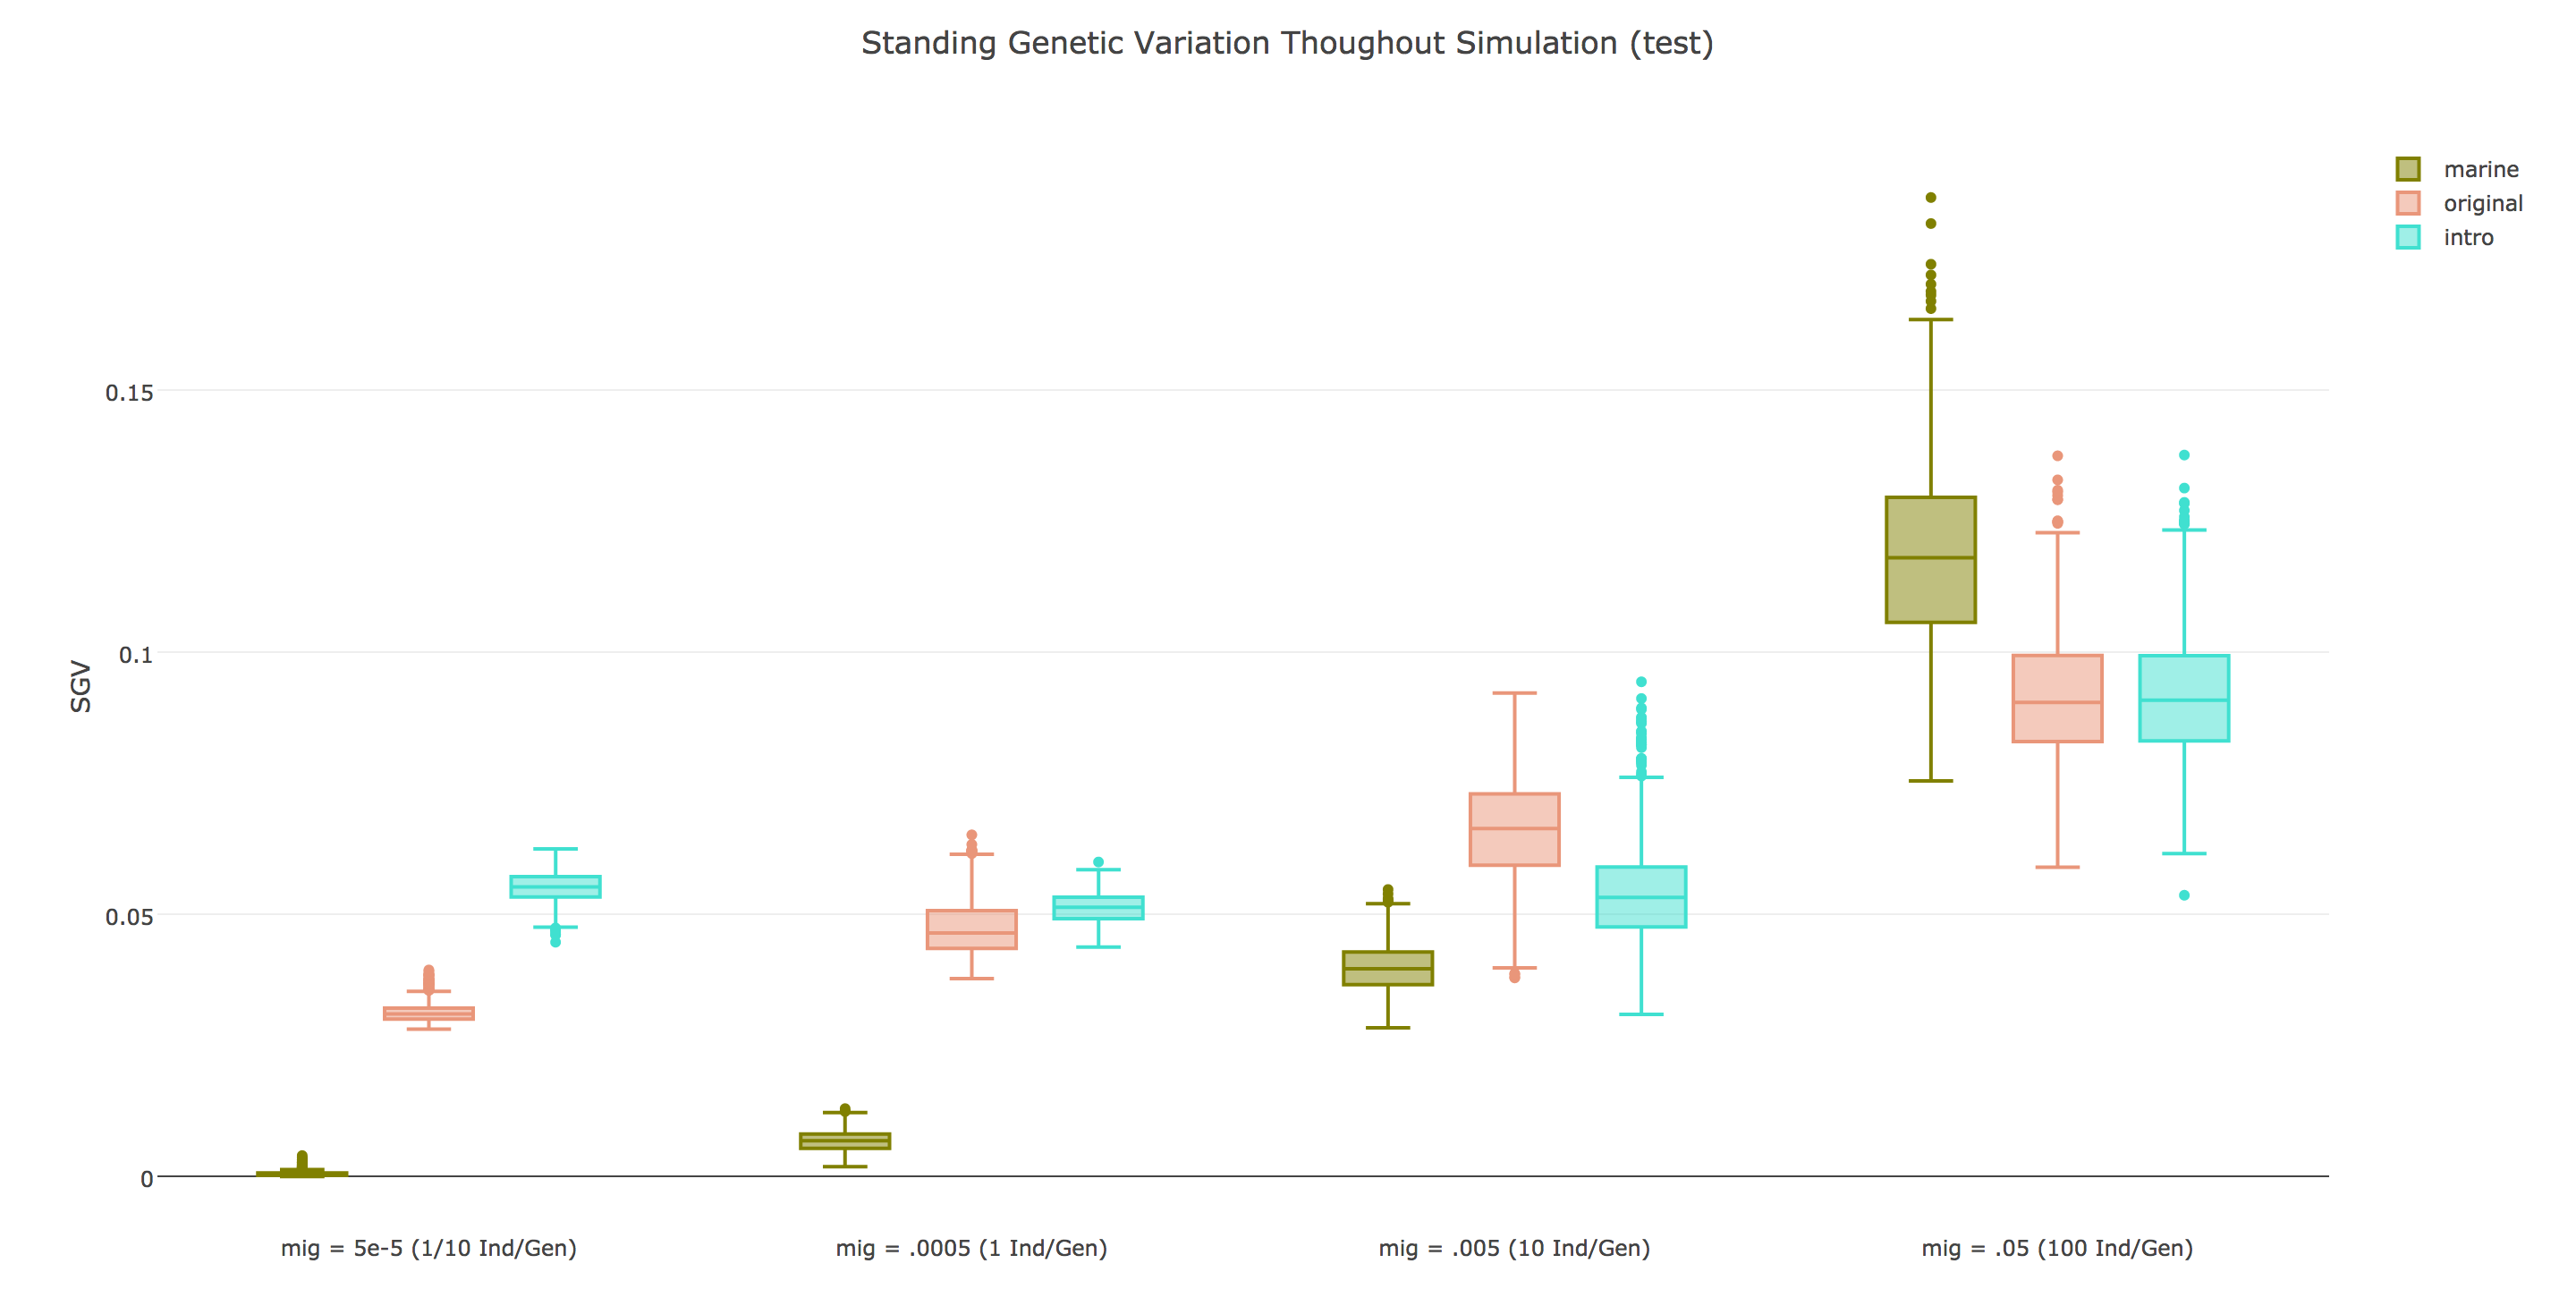
\includegraphics[width=\linewidth]{plotlyPlots/StandingGeneticVariation.png}
  		\caption{(PLACEHOLDER)}
		\label{fig:SGV}
	\end{center}
\end{figure}

\begin{figure}
	\begin{center}
  		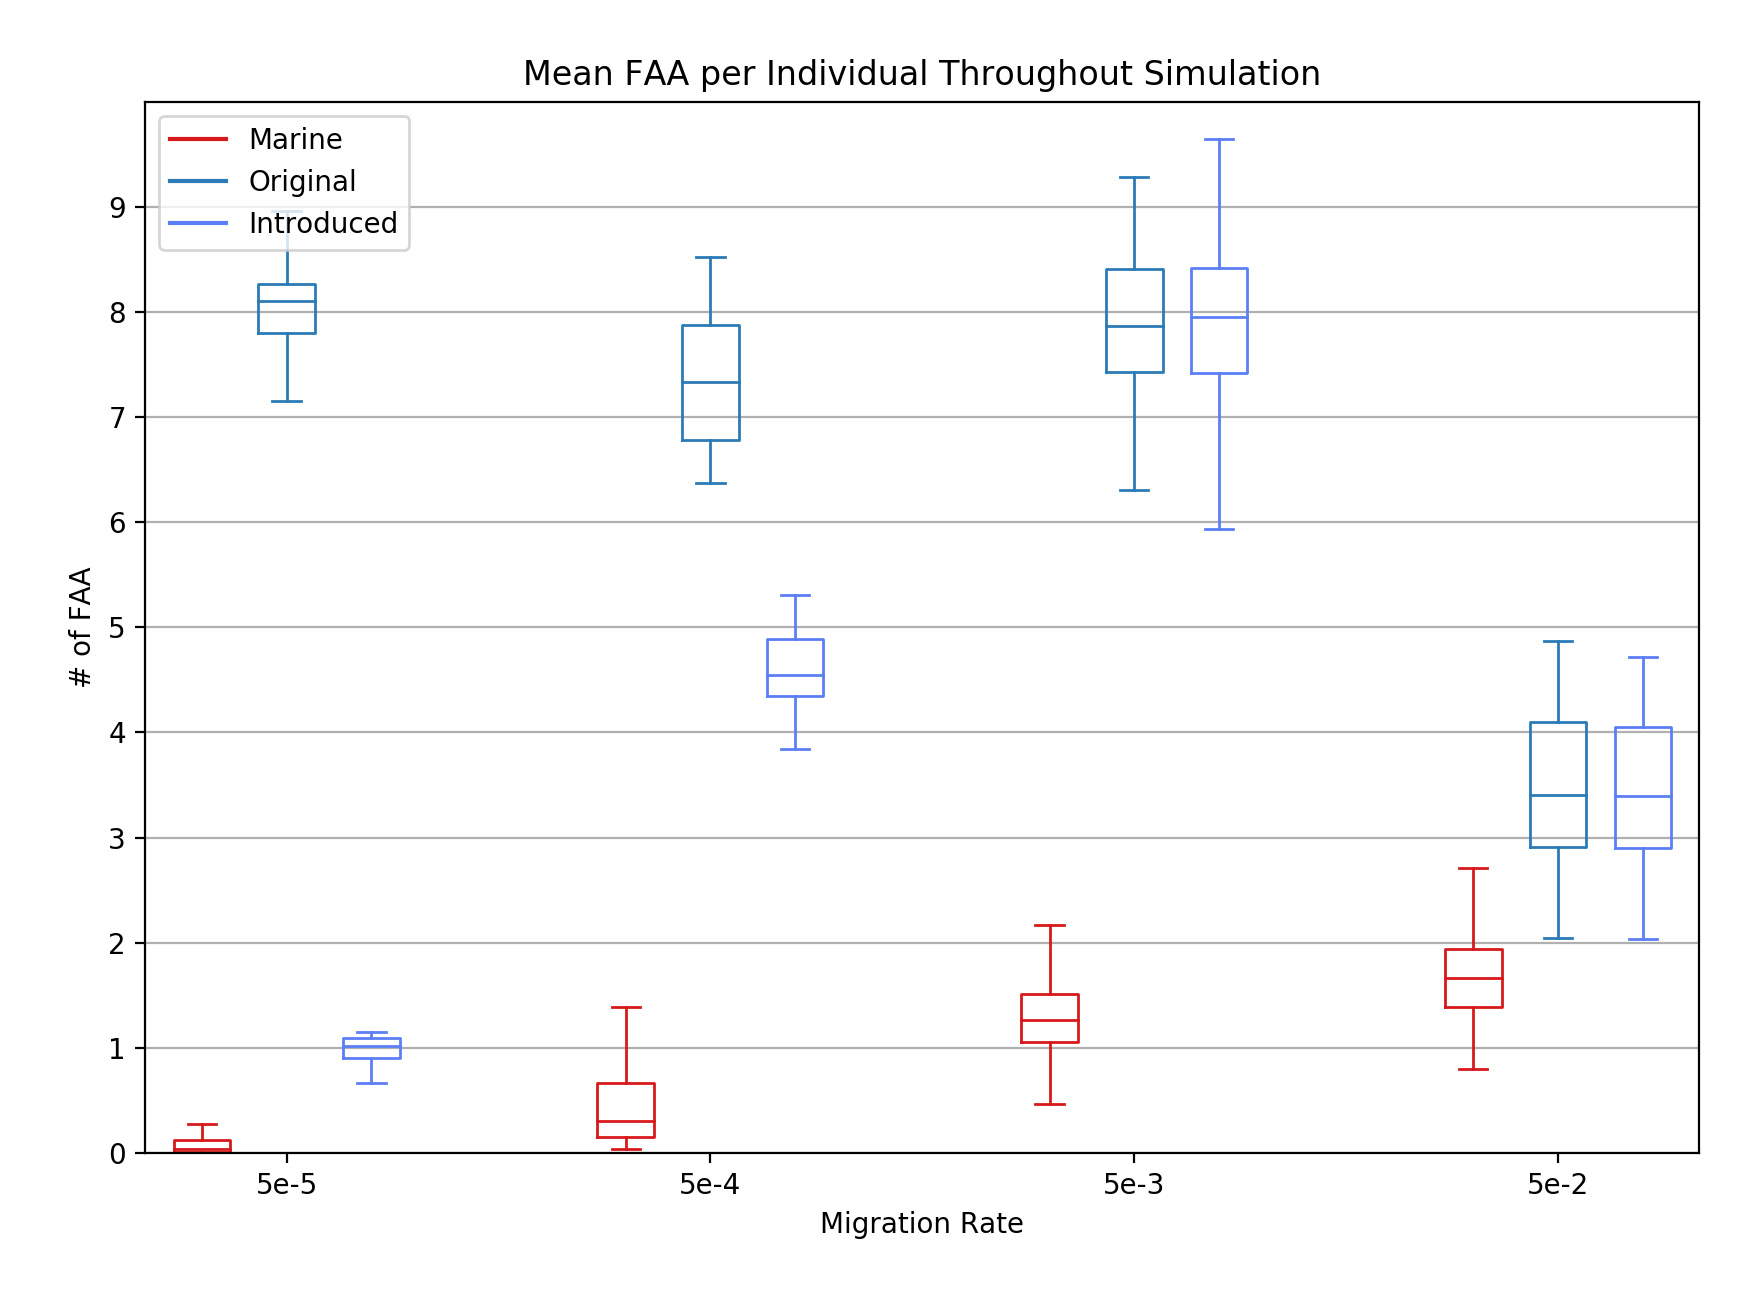
\includegraphics[width=\linewidth]{matplotlibPlots/MFAI.png}
  		\caption{Distributions of mean number of freshwater adapted alleles (FAA) per individual throughout the simulation run, for each subpopulation.
		We count the total number of freshwater alleles for each individual before averaging them in each population and dividing by the total number of defined
		freshwater adapted alleles.
		Looking at total number of FAA per individual gives us an idea behind how many alleles underly a freshwater haplotype, 
		}
  		\label{fig:MNFAI}
	\end{center}
\end{figure}

\begin{figure}
	\begin{center}
  		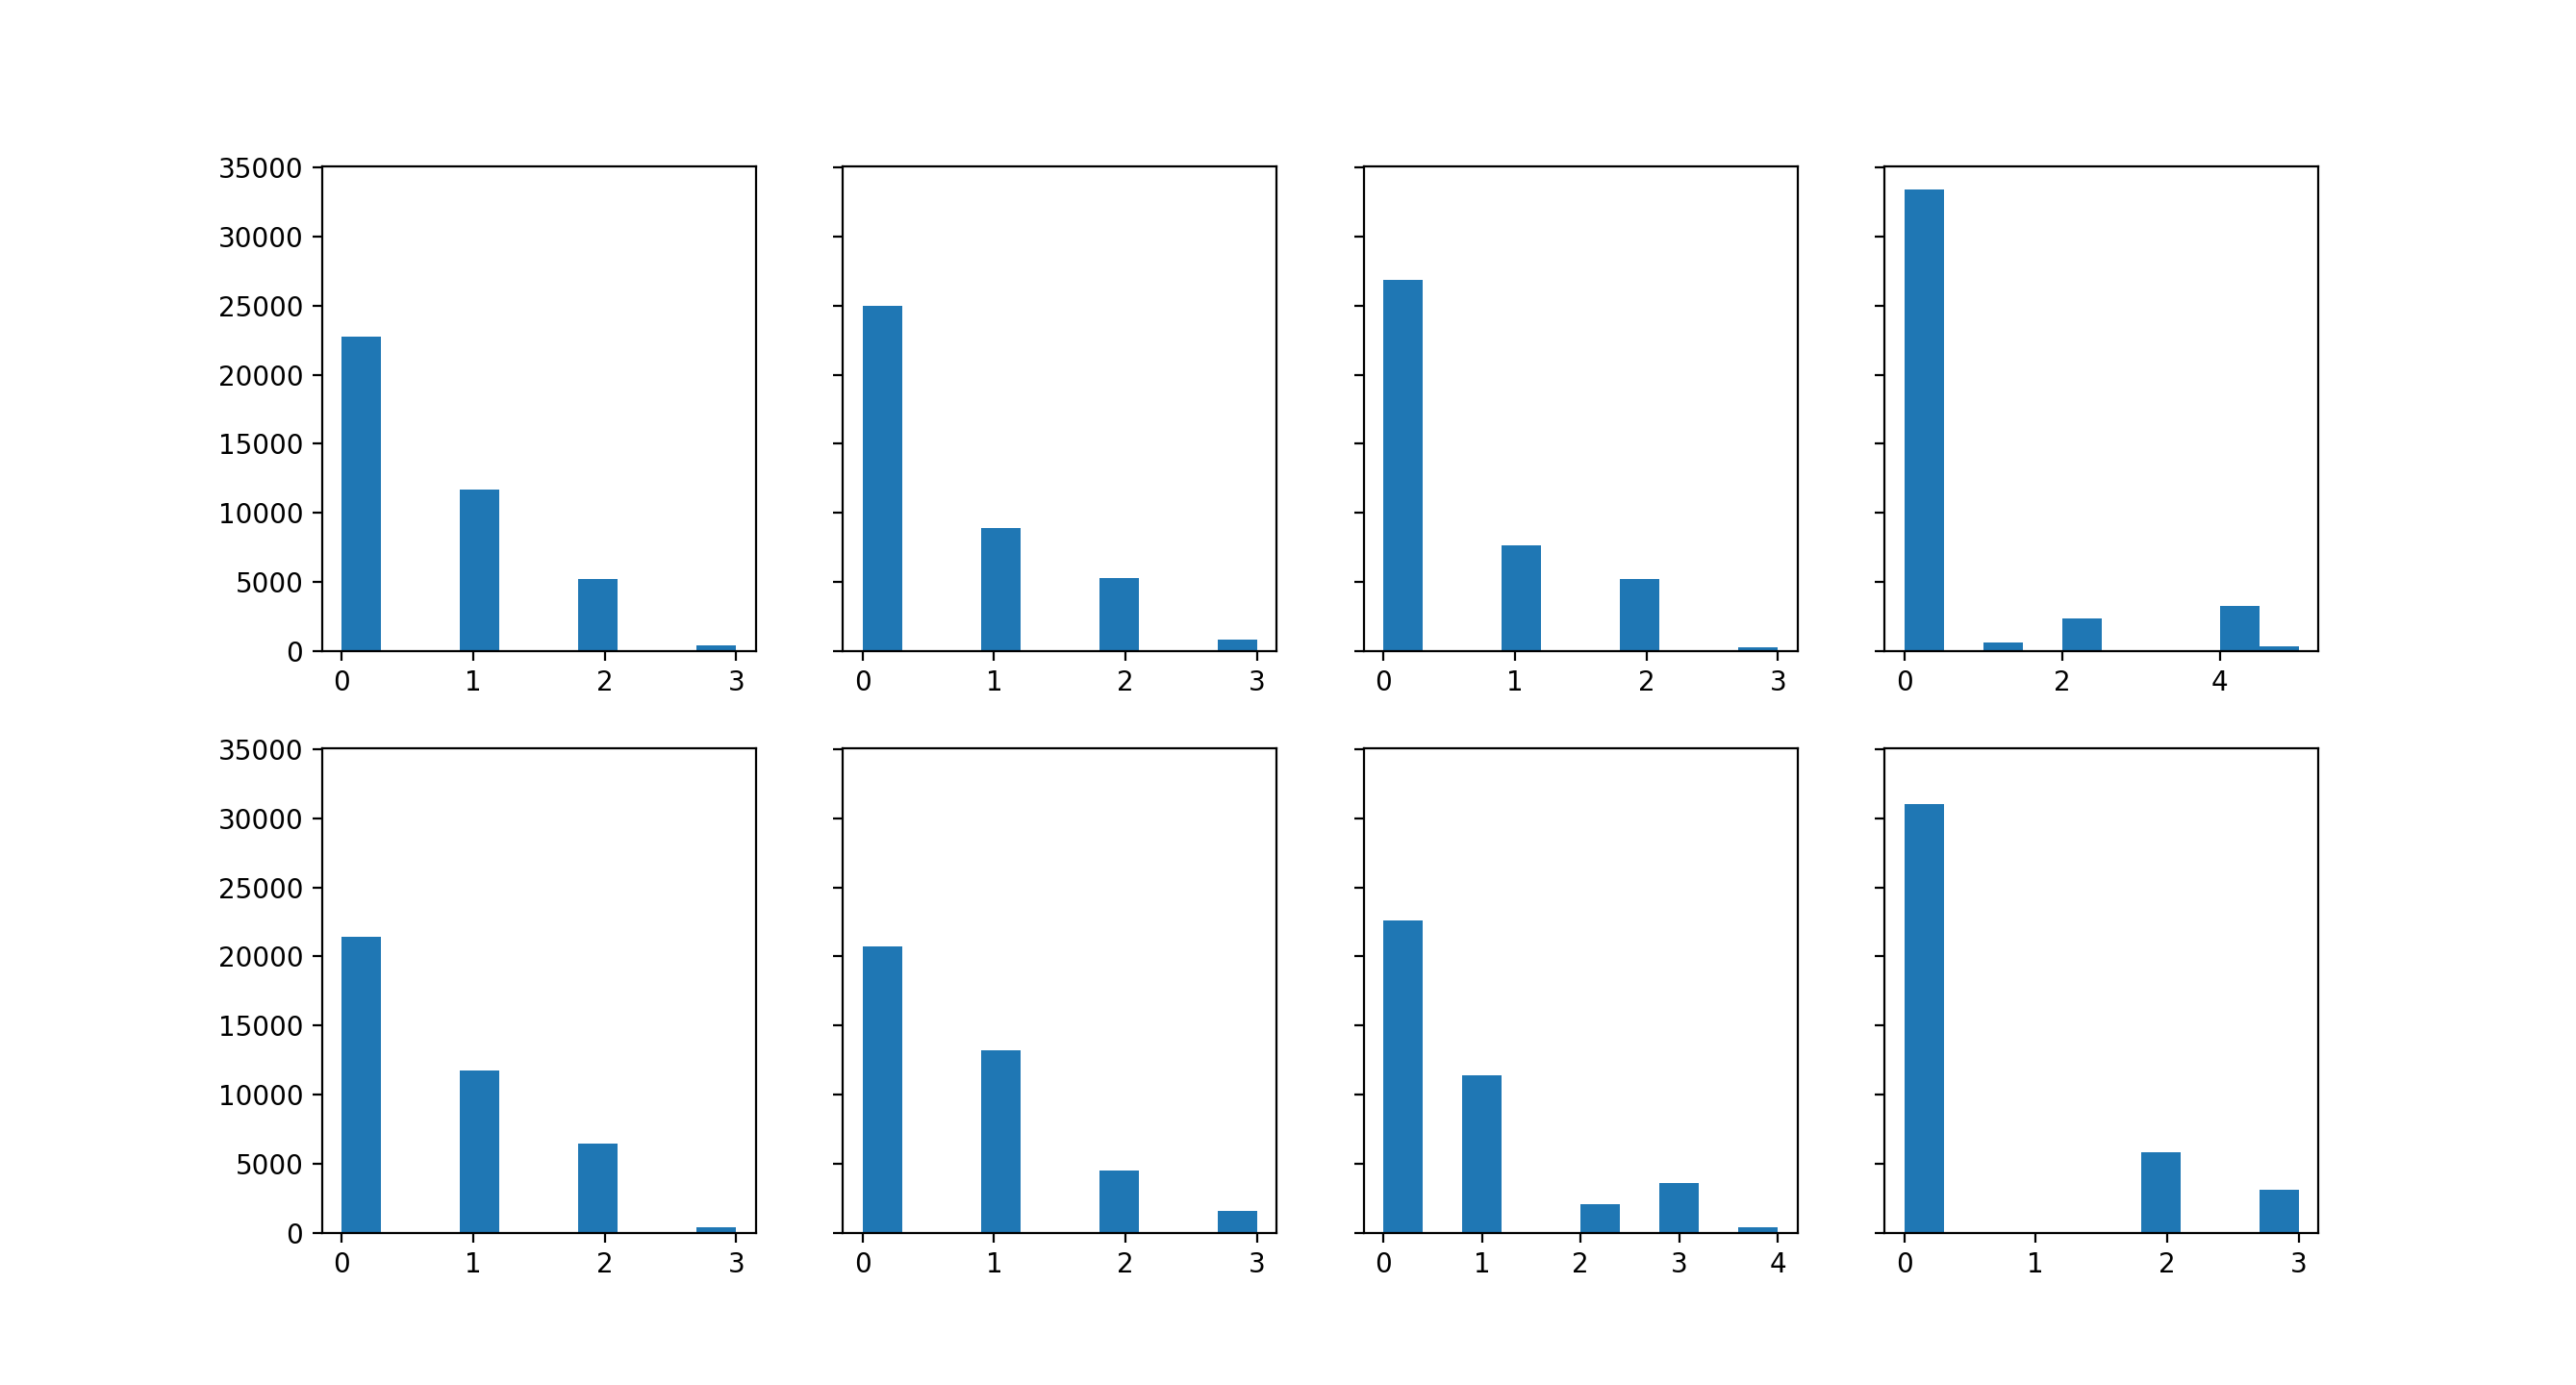
\includegraphics[width=\linewidth]{matplotlibPlots/effectRegionCounts.png}
  		\caption{(PLACEHOLDER)}
		\label{fig:counts}
	\end{center}
\end{figure}

\begin{figure}[h!tb]
	\begin{center}
  		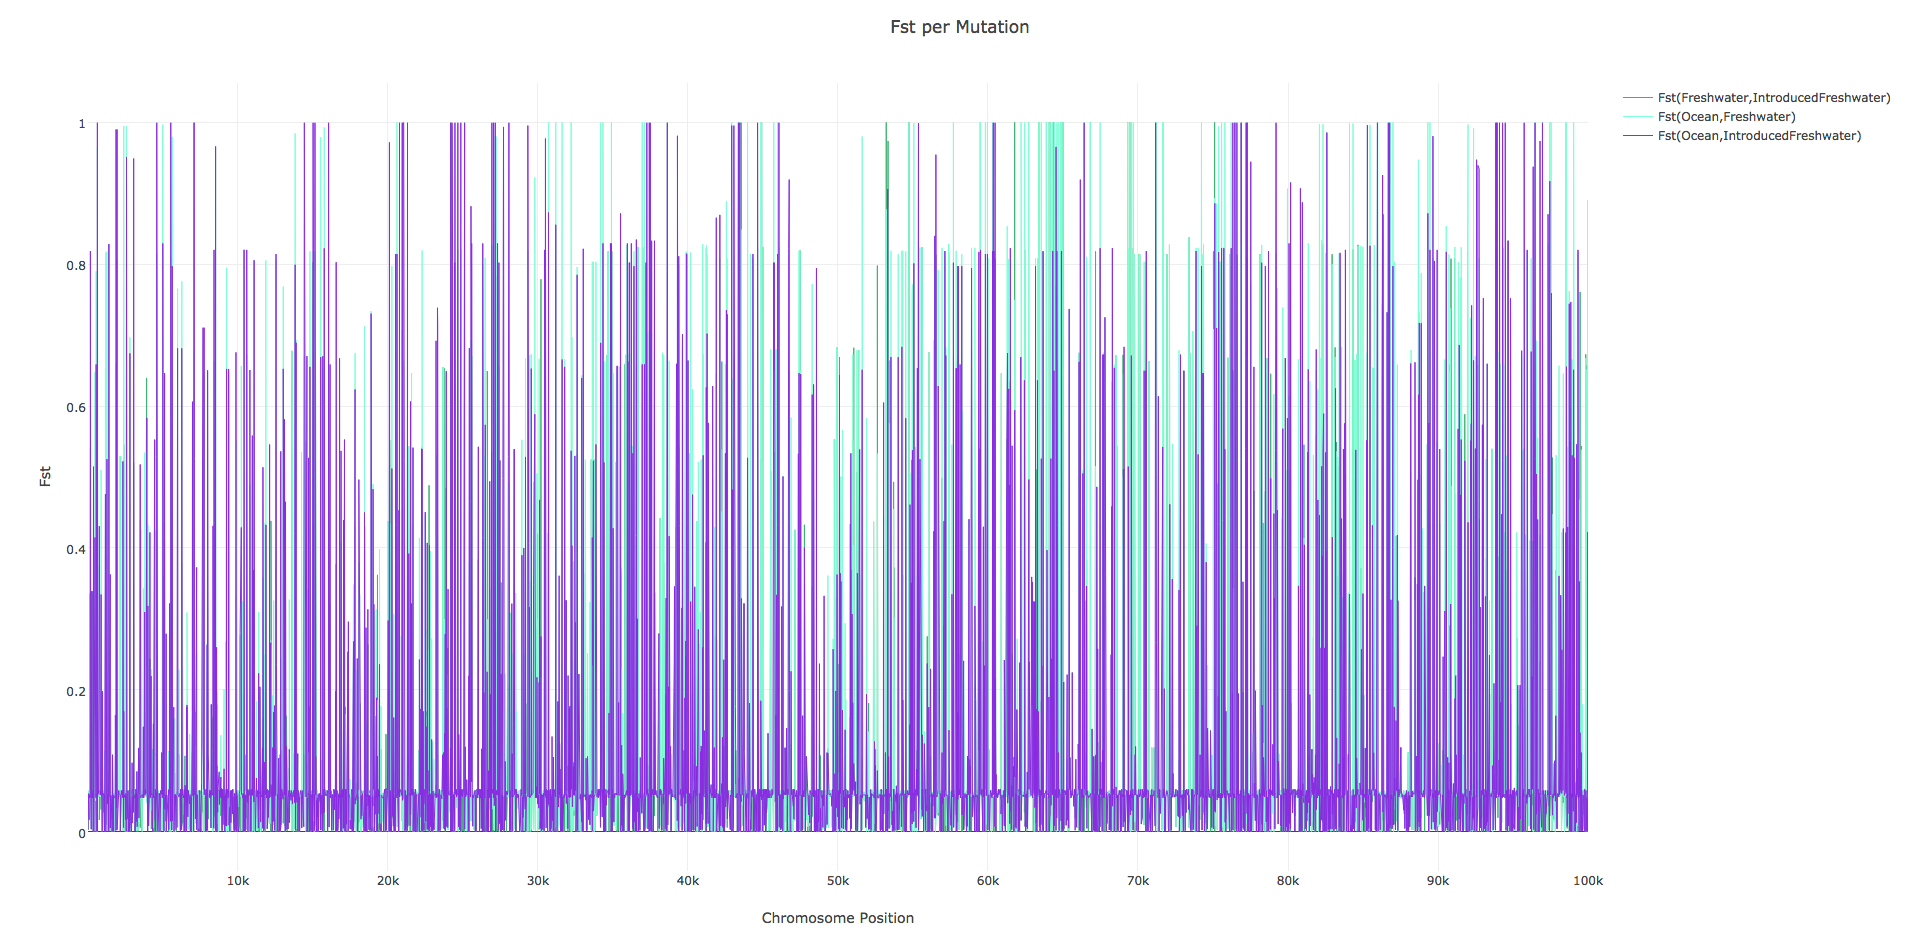
\includegraphics[width=0.7\linewidth]{plotlyPlots/FstAcross5e-5.png}
  		\caption{ (PLACEHOLDER)
		}
  		\label{fig:Fst1}
	\end{center}
\end{figure}

\begin{figure}[h!tb]
	\begin{center}
  		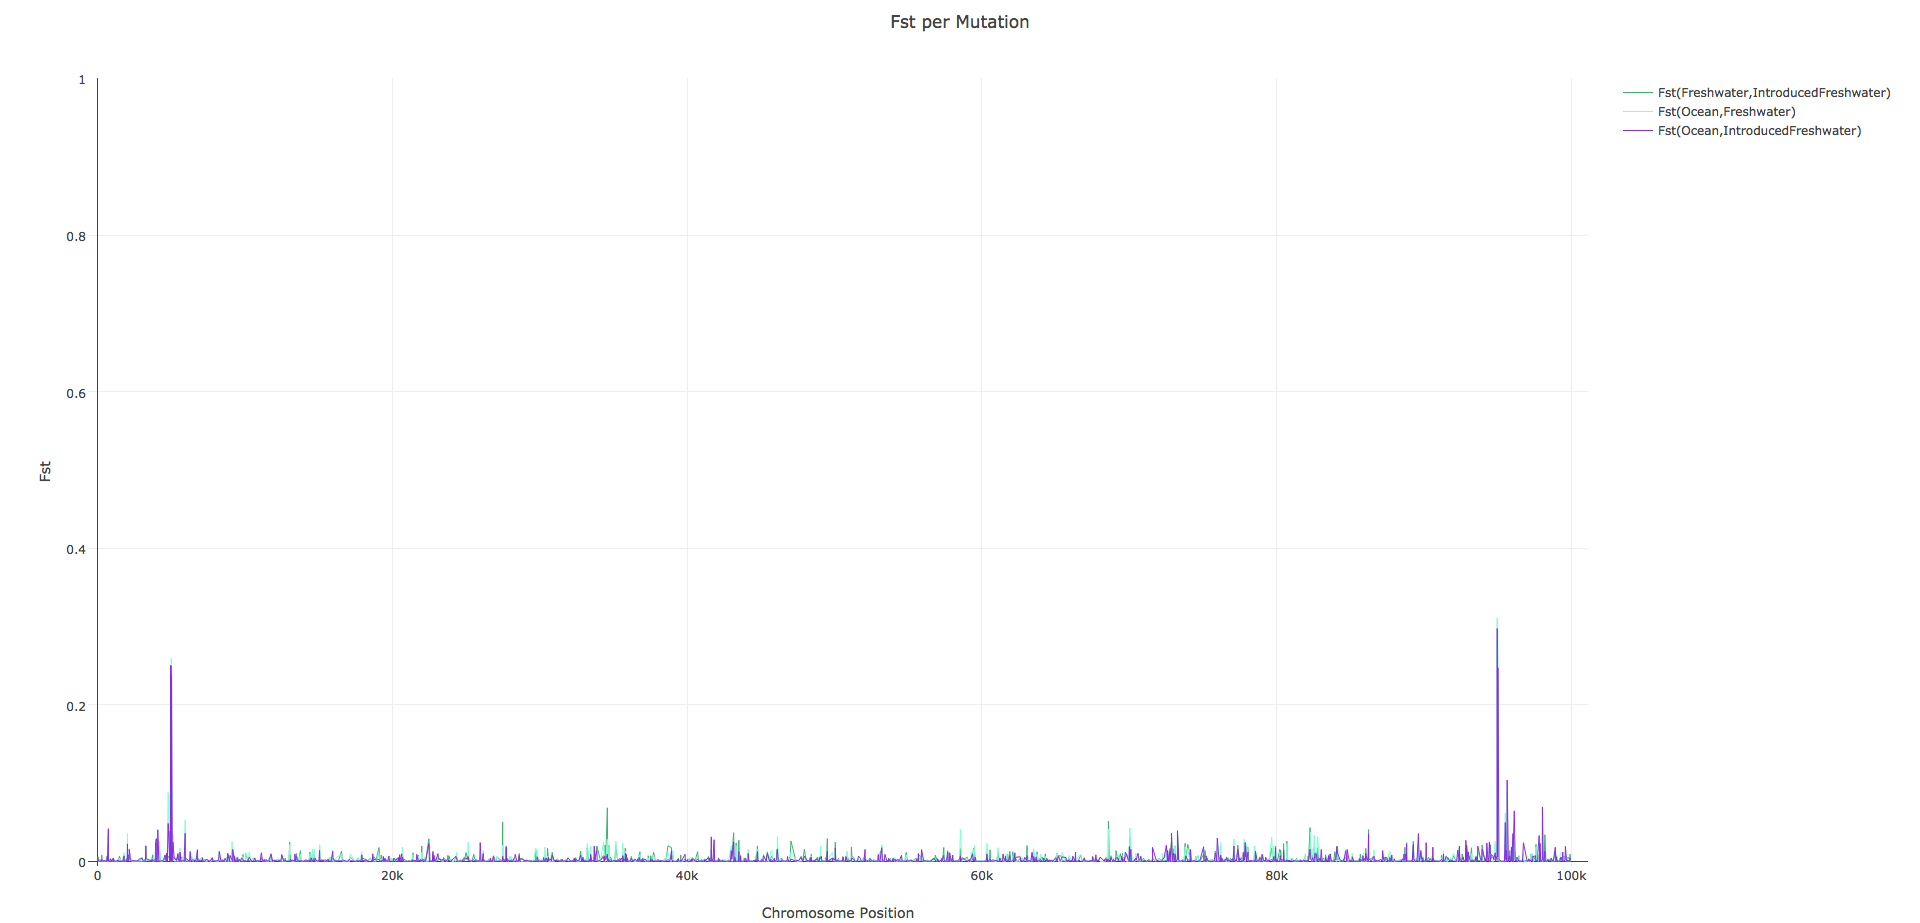
\includegraphics[width=0.7\linewidth]{plotlyPlots/FstAcross5e-2.png}
  		\caption{(PLACEHOLDER)
		}
  		\label{fig:Fst4}
	\end{center}
\end{figure}

\begin{figure}[h!tb]
	\begin{center}
  		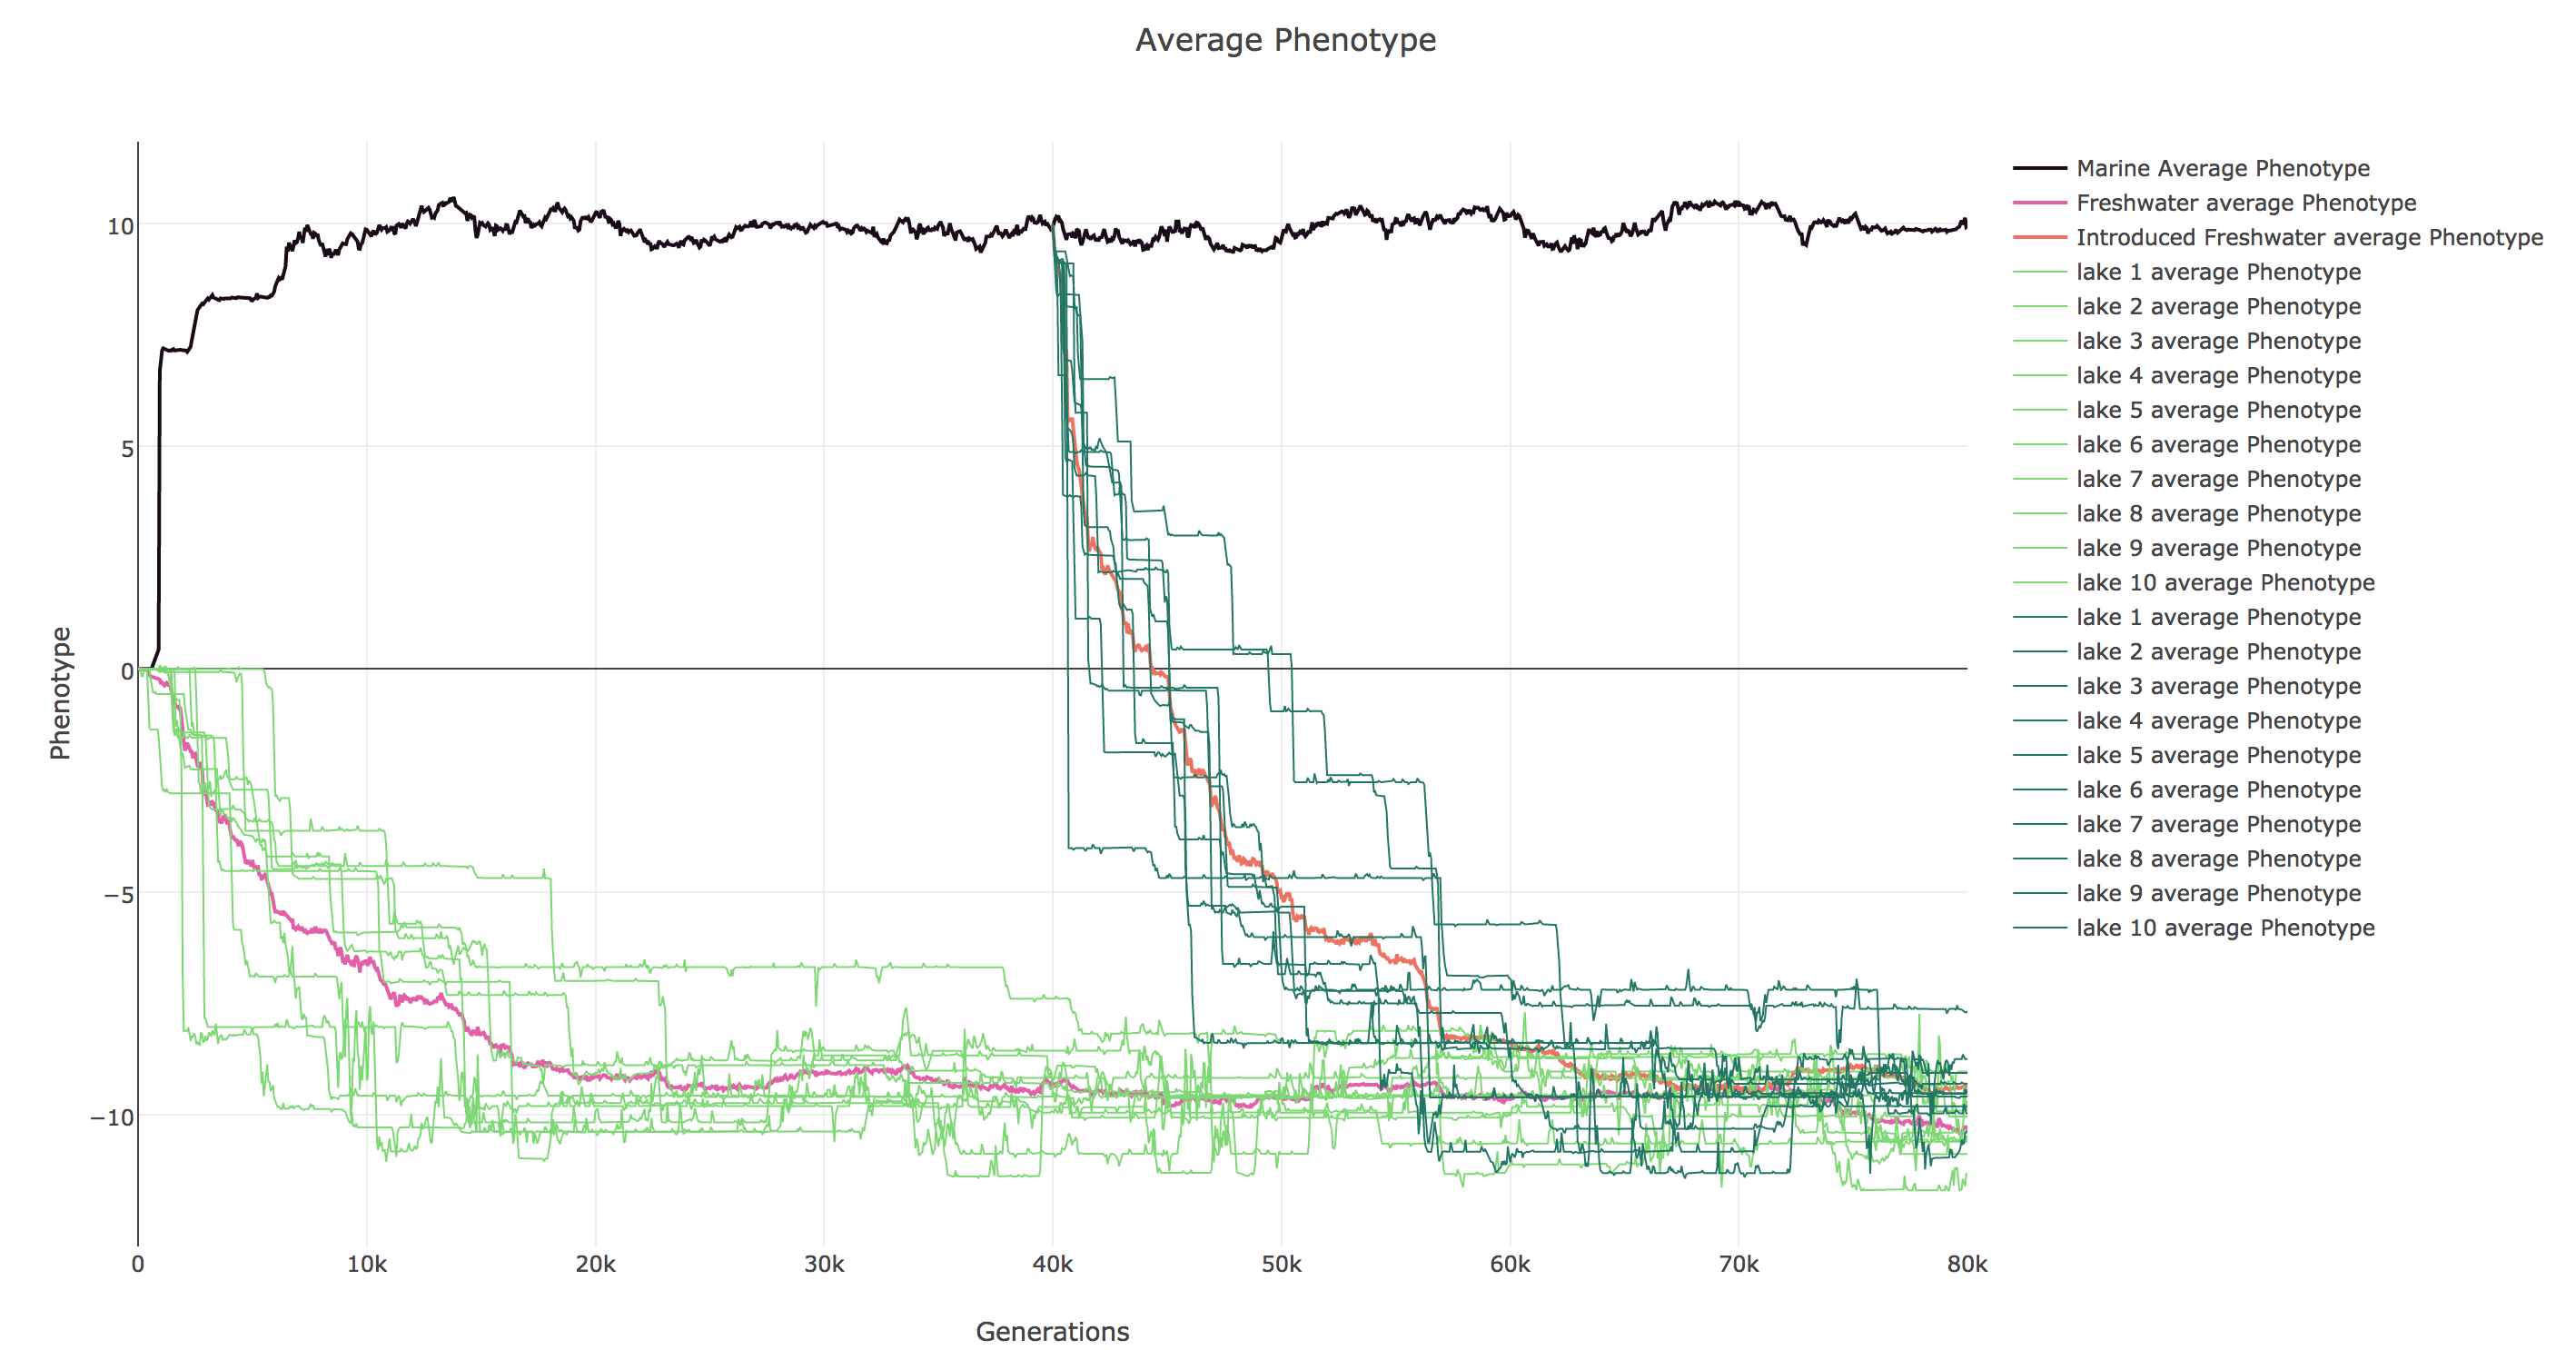
\includegraphics[width=0.7\linewidth]{plotlyPlots/PhenotypeThroughout5e-5.png}
  		\caption{ (PLACEHOLDER)
		}
  		\label{fig:phenotype_ts1}
	\end{center}
\end{figure}

\begin{figure}[h!tb]
	\begin{center}
  		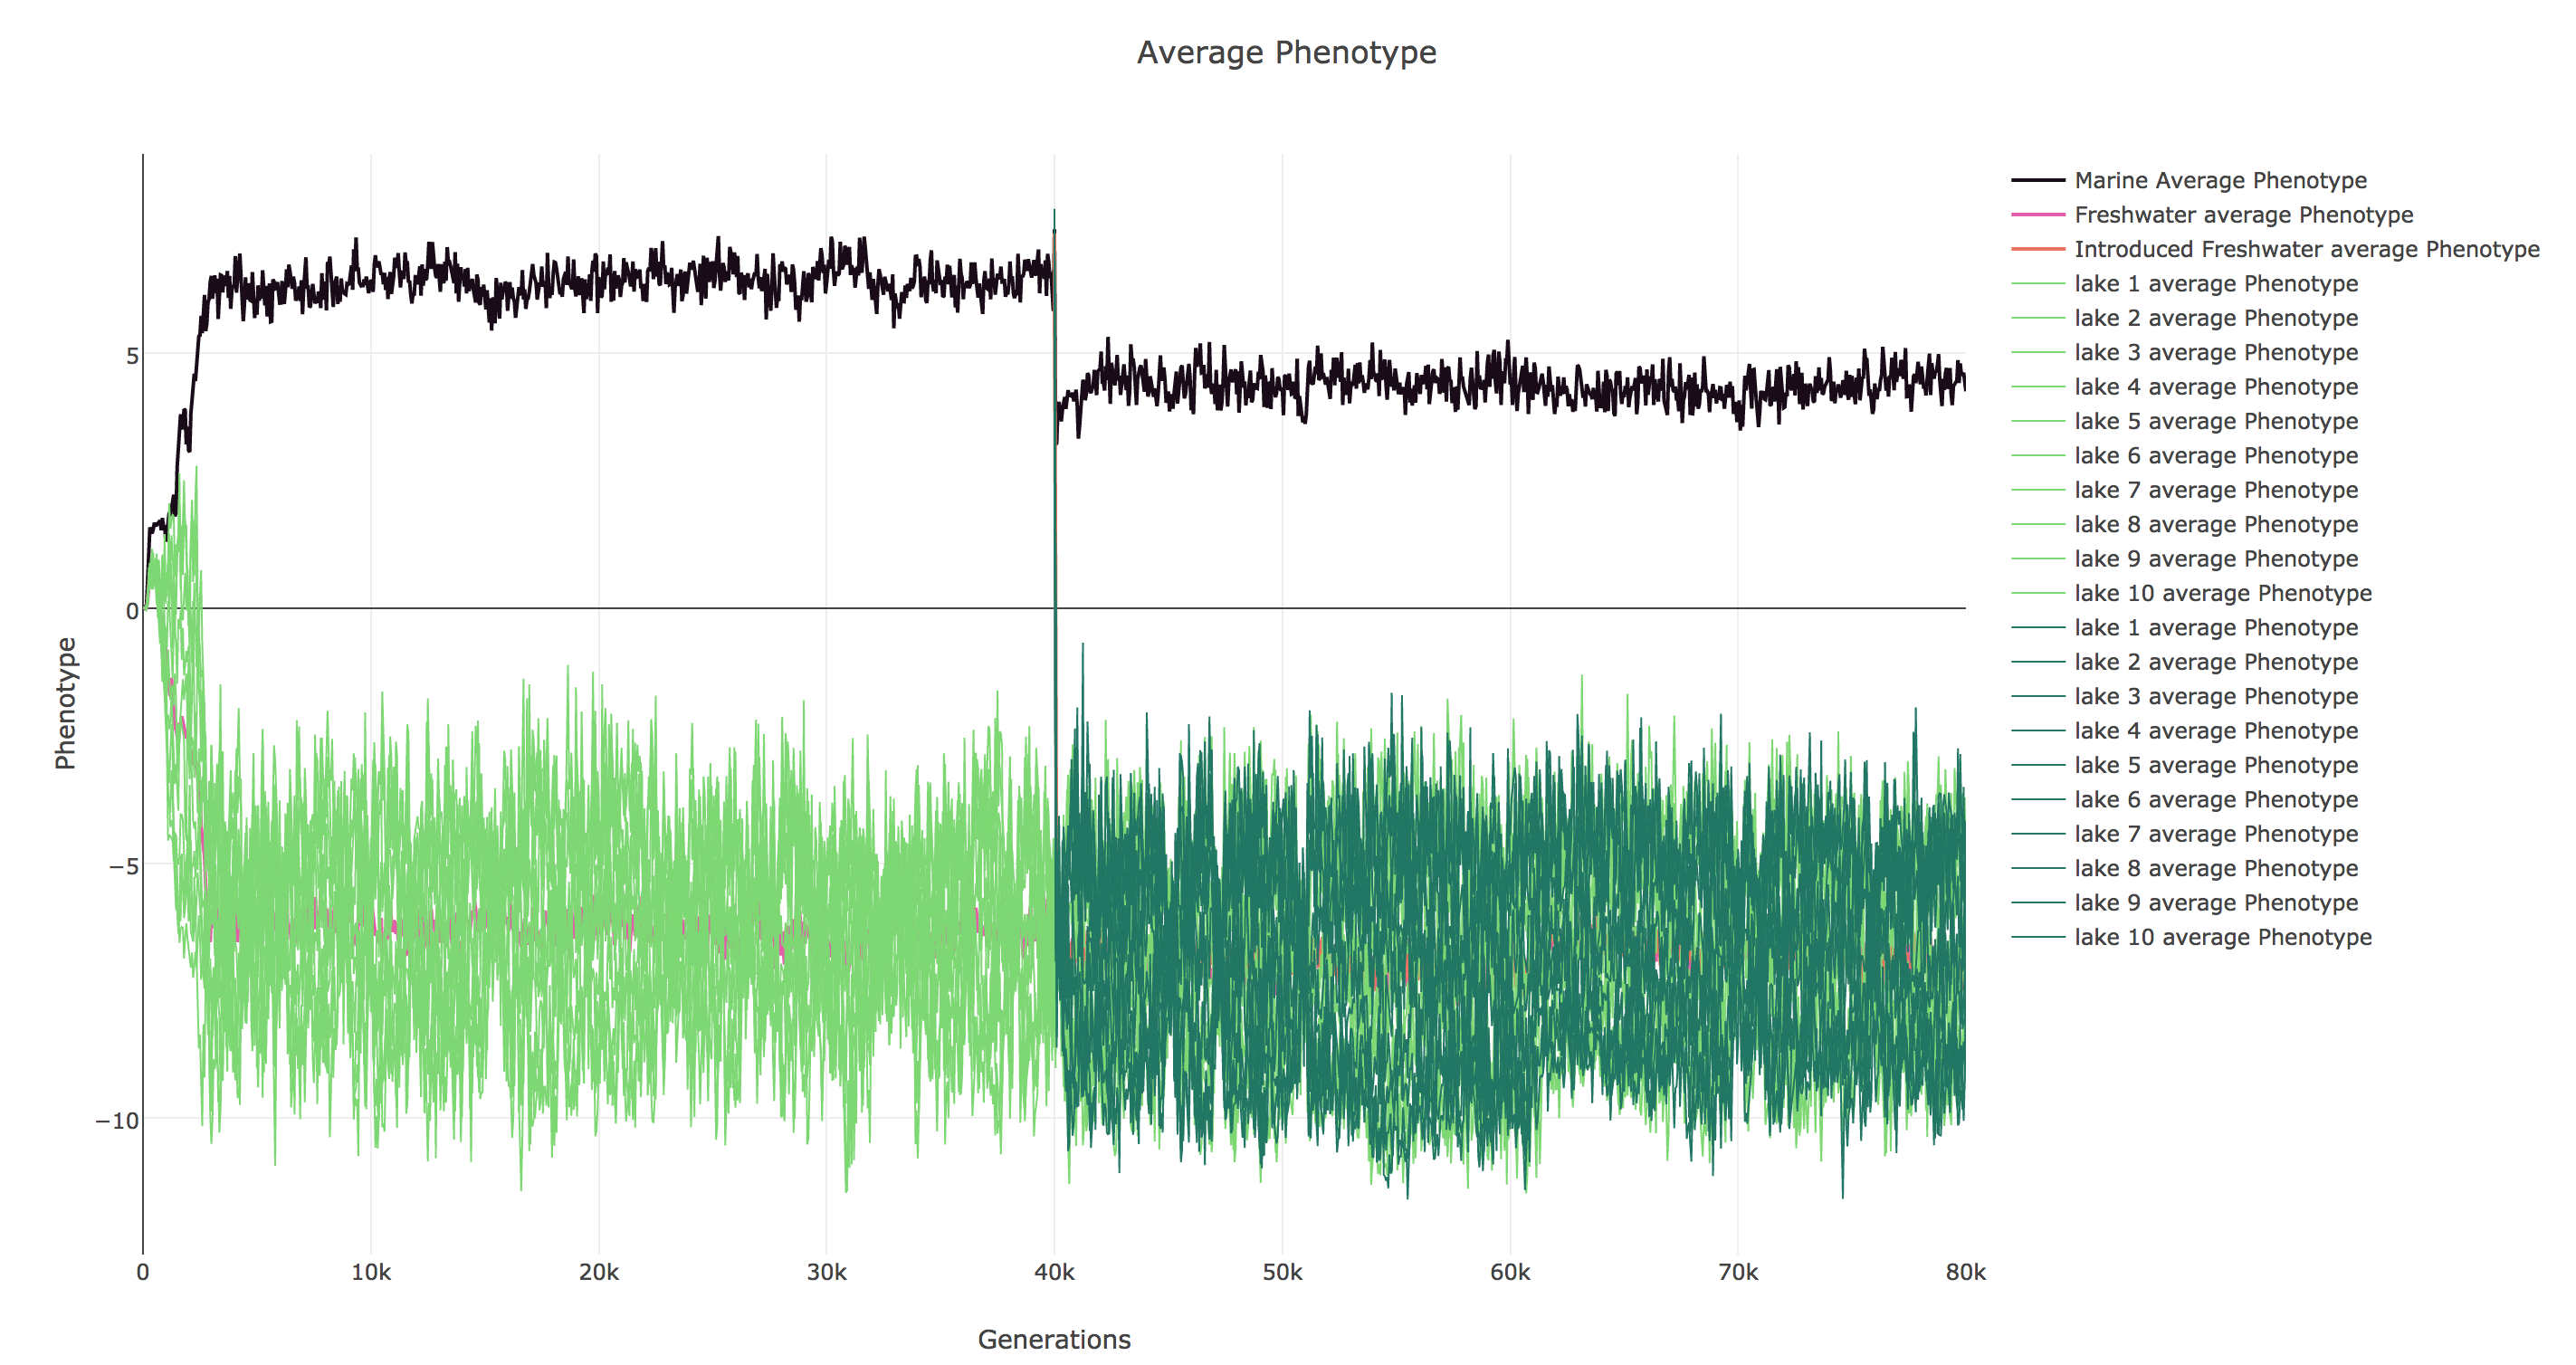
\includegraphics[width=0.7\linewidth]{plotlyPlots/PhenotypeThroughout5e-2.png}
  		\caption{(PLACEHOLDER)
		}
  		\label{fig:phenotype_ts4}
	\end{center}
\end{figure}



\end{document}
